\documentclass[12]{article}
\usepackage{prettyref}
\usepackage[left=2cm,right=2cm,top=2cm,bottom=2cm]{geometry}
\usepackage{graphicx}
\usepackage{amsmath, amssymb}
\usepackage{mathtools}
\usepackage{physics}
\usepackage{textcomp}
\usepackage{float}
\usepackage[british]{babel}
\usepackage{hhline}
\usepackage{multirow}
\usepackage{hyperref}
\hypersetup{
    colorlinks=true,
    linkcolor=blue,
    filecolor=magenta,      
    urlcolor=cyan,
}
\begin{document}
\begin{center}
\begin{Huge}
RESULTS-Anti-ferromagnetic Trigger
\end{Huge}
\end{center}
%\chapter{Results}\label{ch:A}
This chapter will focus on the effects on the performance of quantum annealing algorithm upon adding the second trigger, namely the anti-ferromagnetic trigger, to the original Hamiltonian. Unlike in the case of the ferromagnetic trigger, for anti-ferromagnetic trigger the strength parameter, g in equation (\ref{eq:b12}) plays a more decisive role than merely controlling the extent by which the minimum gap is enlarged. The anti-ferromagnetic trigger alters the energy spectra, the minimum energy gaps, and the number of anti-crossings between the ground and first excited energy state of the Hamiltonian, depending on the strength with which the trigger is added, as well as on the problem itself. We shall begin by observing the effects of adding the anti-ferromagnetic trigger to the original Hamiltonian, for the three chosen problems. The following sections will then showcase the role that the strength parameter - g plays.

\section*{The chosen problems}
Let us begin by considering the first chosen case, with largest success probability. 
Figure (\ref{fig:a1}), (\ref{fig:a2}) and (\ref{fig:a3}) shows the energy spectrum and the instantaneous energy values after adding the anti-ferromagnetic trigger to the first chosen case, with strengths 0.5, 1 and 2 respectively.
\begin{figure}[H]
\centering 
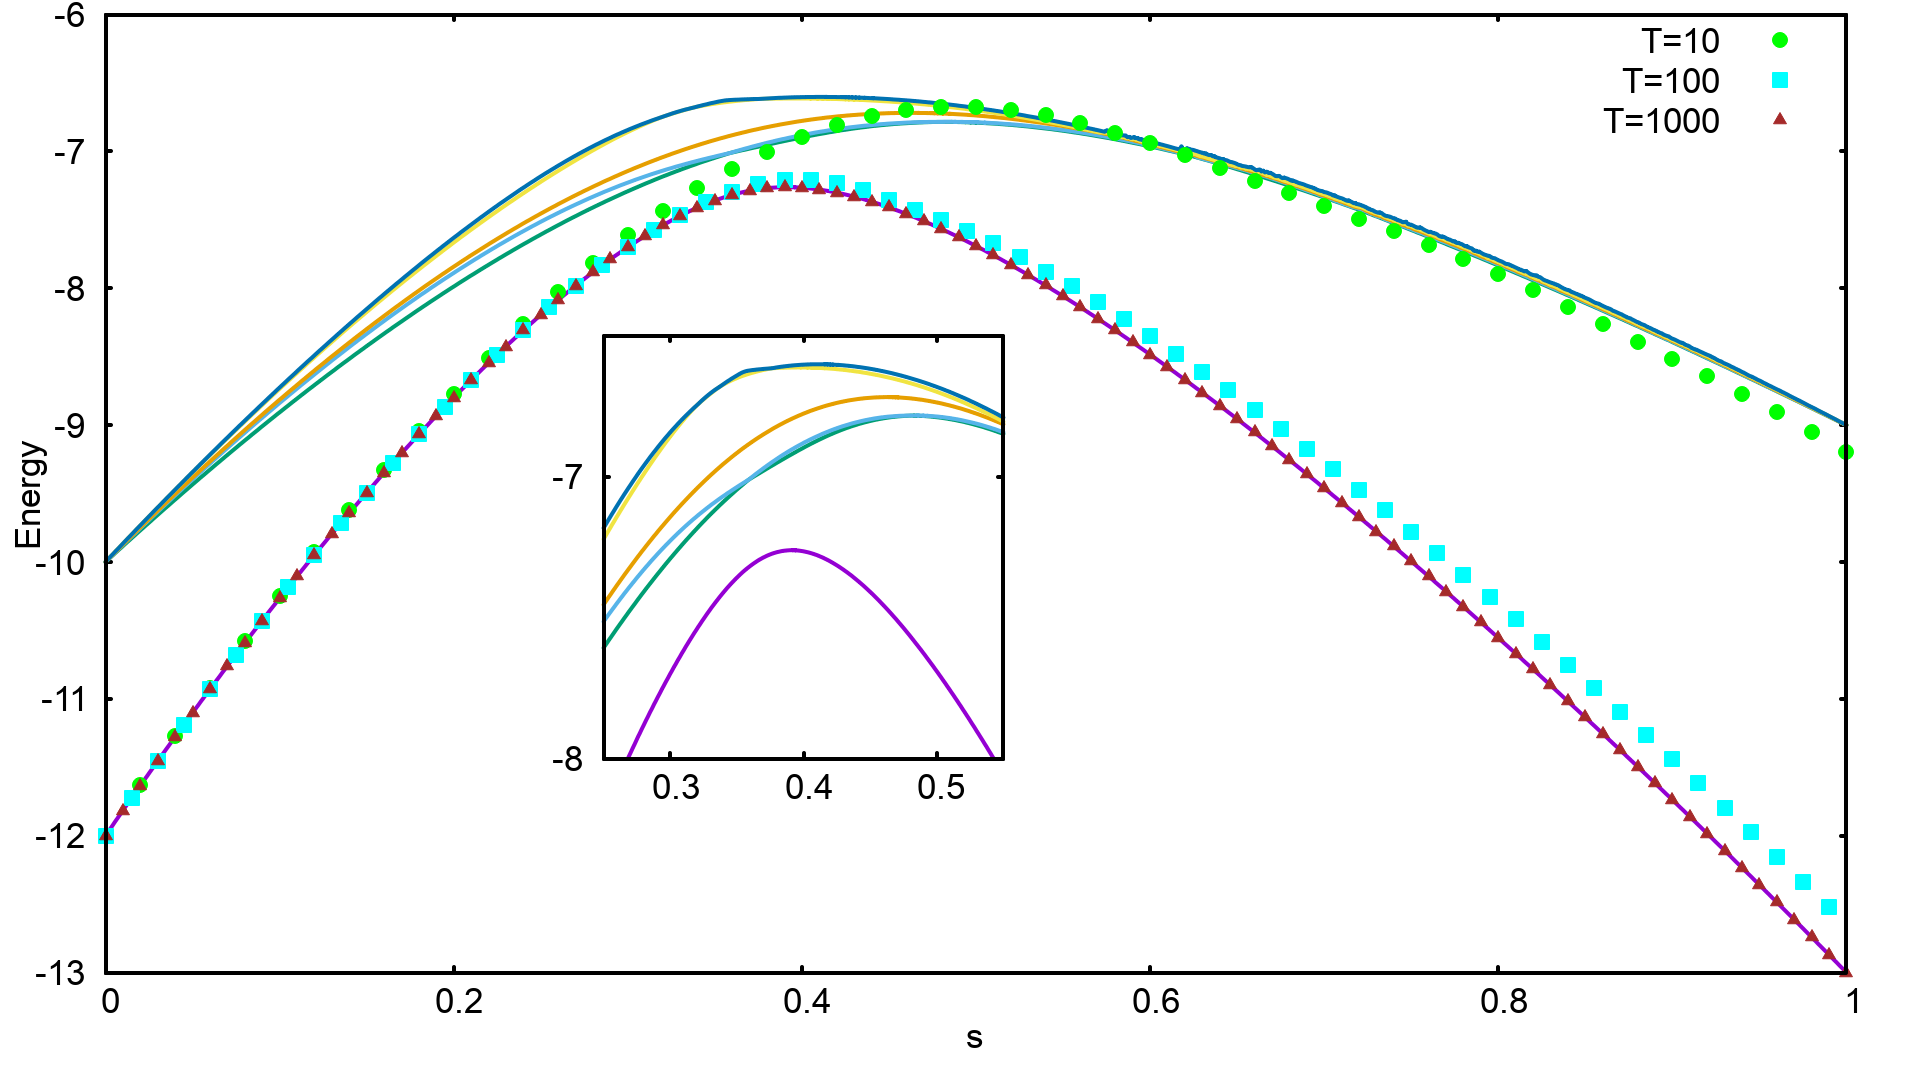
\includegraphics[scale=0.3]{733_s12_A_g0.png}
\caption{The energy spectrum for the first problem, with instantaneous energy values corresponding to three annealing times, with Anti-ferromagnetic trigger, and g=0.5. $\Delta_{min}$ was found to be 0.3070, while $p$=0.9117 for $T_A$=100. }
\label{fig:a1}
\end{figure}
\begin{figure}[H]
\centering 
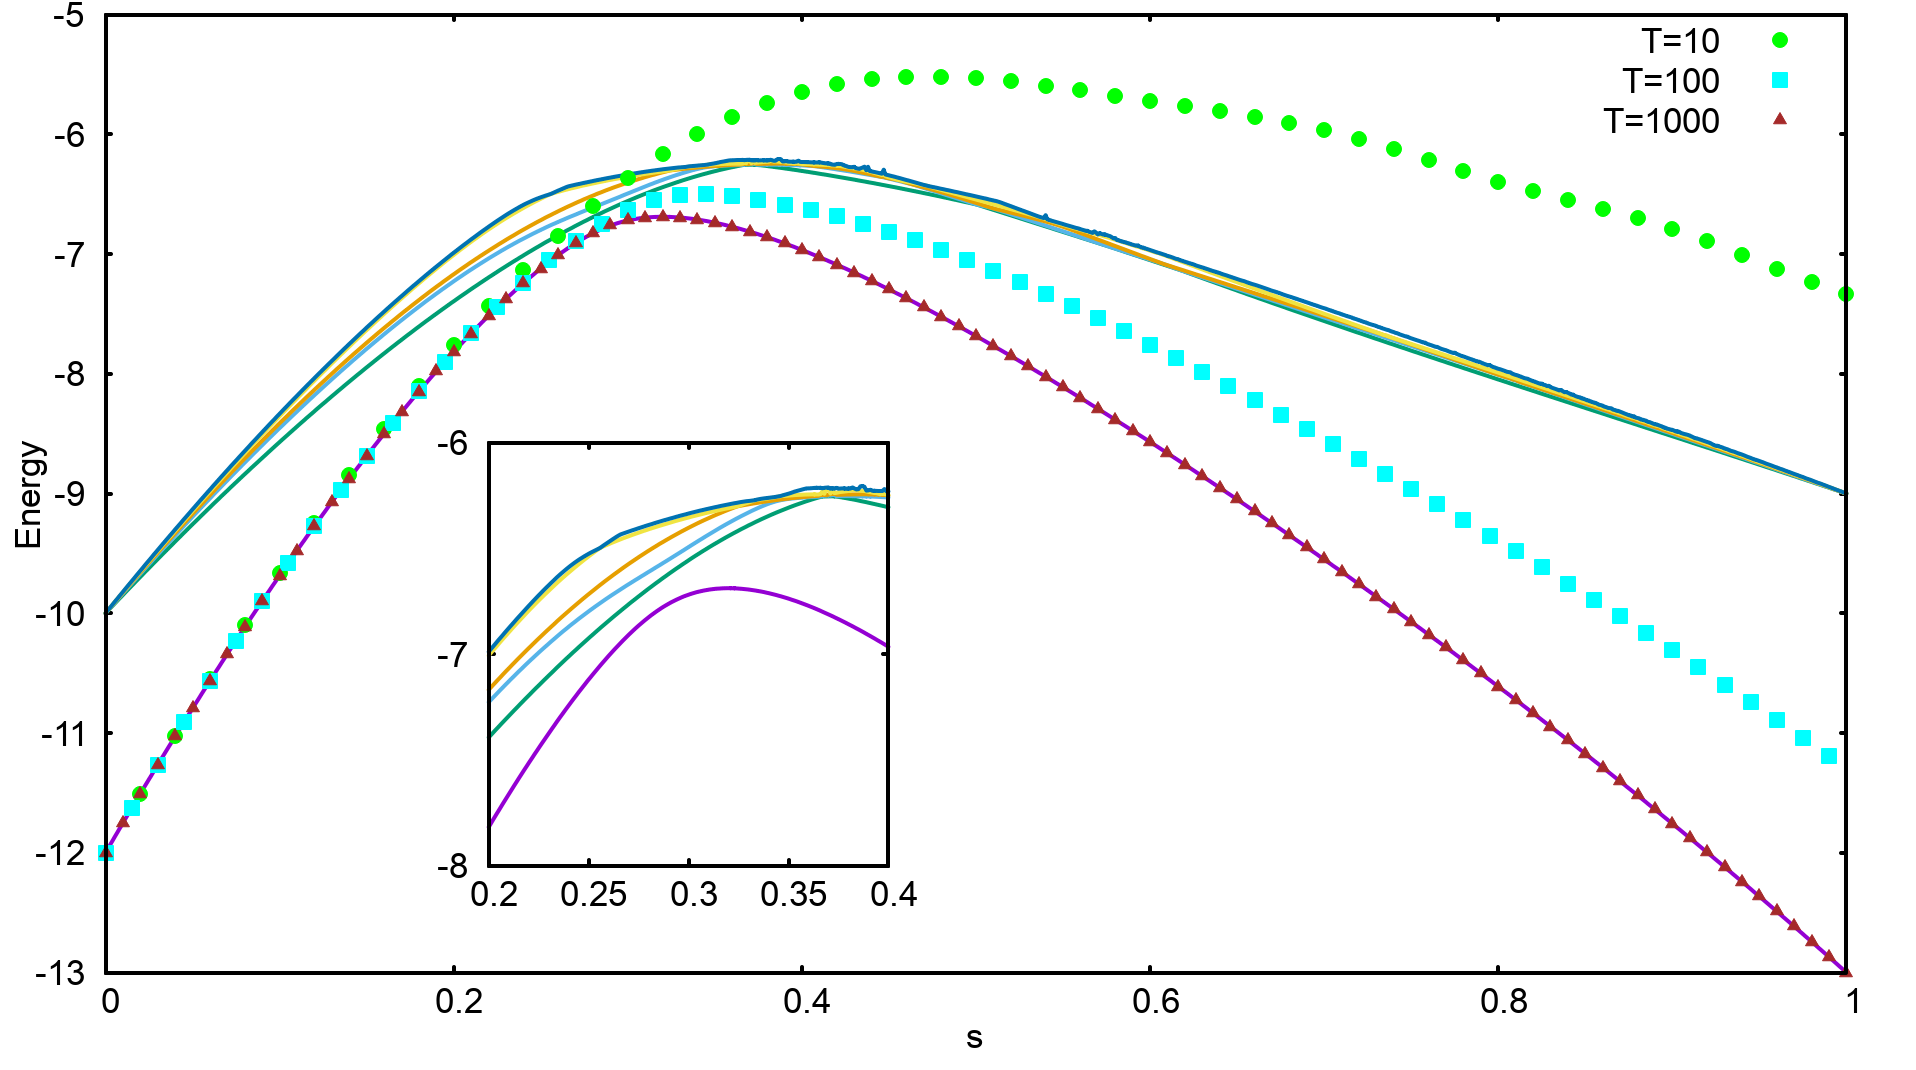
\includegraphics[scale=0.3]{733_s12_A_g1.png}
\caption{The energy spectrum for the first problem, with instantaneous energy values corresponding to three annealing times, with Anti-ferromagnetic trigger, and g=1. $\Delta_{min}$ was found to be 0.1349, while $p$=0.5747 for $T_A$=100. }
\label{fig:a2}
\end{figure}
\begin{figure}[H]
\centering 
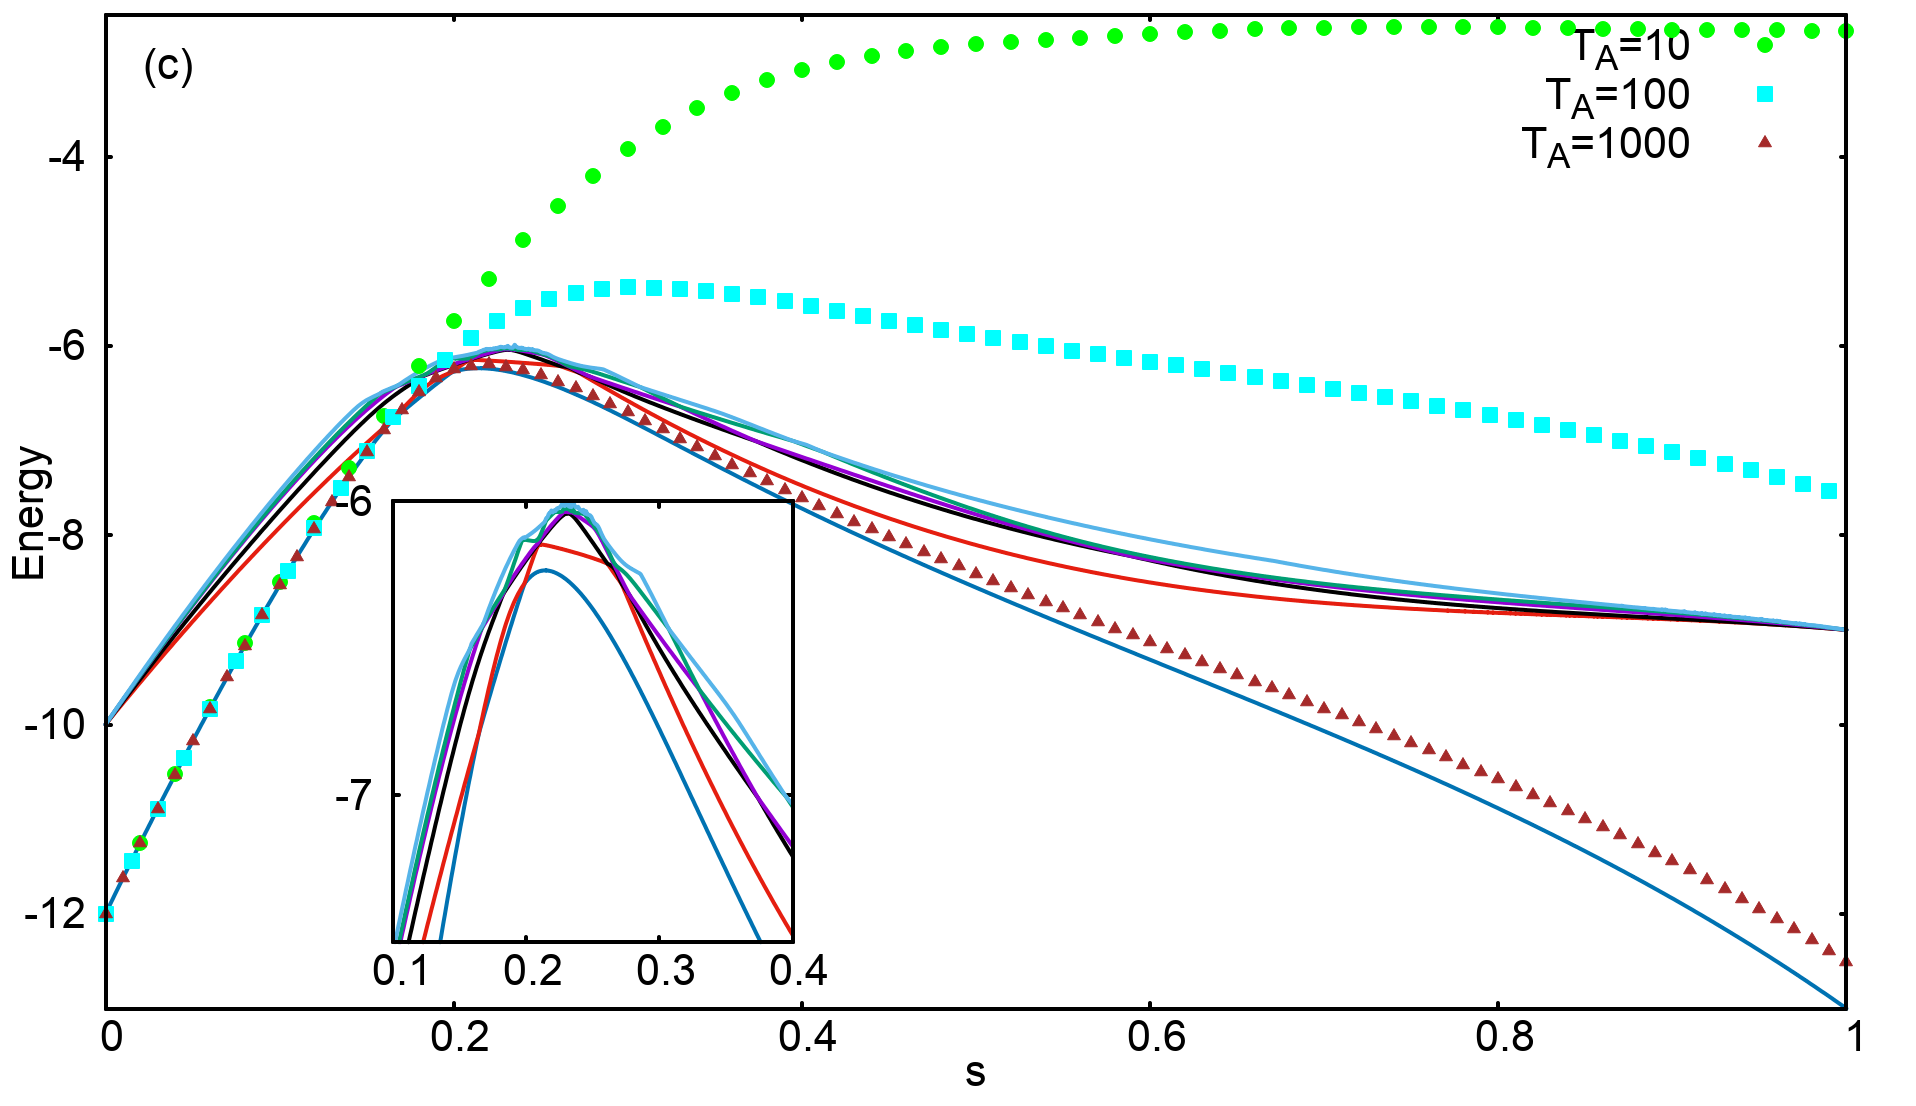
\includegraphics[scale=0.3]{733_s12_A_g2.png}
\caption{The energy spectrum for the first problem, with instantaneous energy values corresponding to three annealing times, with Anti-ferromagnetic trigger, and g=2. $\Delta_{min}$ was found to be 0.0020, while $p$=0.0273 for $T_A$=100. }
\label{fig:a3}
\end{figure}
Table (\ref{tab:a1}) shows a comparison of the success probabilities - p, and minimum energy gaps - $\Delta_{min}$ between the original Hamiltonian and the Hamiltonian after adding the anti-ferromagnetic triggers with different strengths.

\begin{table}[H]
\centering
\renewcommand{\arraystretch}{1.5}
\begin{tabular}{|c|c|c|c|c|}
\hline 
CASE 1 & Original Hamiltonian & Trigger=A, g=0.5 & Trigger=A, g=1 & Trigger=A, g=2 \\ 
\hline 
$\Delta_{min}$ & 0.4407 & 0.3070 & 0.1349 & 0.0020 \\ 
\hline 
p($T_A$=10) & 0.3444 & 0.1446 & 0.0279 & 1.271 $\times 10^{-4}$ \\ 
\hline 
p($T_A$=100) & 0.0044 & 0.9117 & 0.5747 & 0.0273 \\ 
\hline 
p($T_A$=1000) & 0.9999 & 0.9999 & 0.9999 & 0.8761 \\ 
\hline 
s value at $\Delta_{min}$ & 0.459 & 0.367 & 0.282 & 0.254 \\ 
\hline
Number of anti-crossings & 1 & 2 & 1 & 4 \\
\hline
\end{tabular} 
\caption{A comparison of the minimum gaps and the success probabilities for the first chosen case, between the original Hamiltonian and and the Hamiltonian with anti-ferromagnetic trigger (A) of different strengths. The minimum gaps become succesively smaller as the strength of the anti-ferromagnetic trigger is increased. The success probabilities are decreased as a result. The value of s corresponding to the position of the minimum gap also becomes smaller.}
\label{tab:a1}
\end{table}
As can be noted from the table above, the minimum energy gap decreases upon adding the ferromagnetic trigger, and this decrease becomes larger as the strength of the trigger is increased. Consequently, the success probabilities are found to be decreasing as well. The value of annealing parameter - s also become smaller with increasing strength of the trigger.
A new feature observed after adding the anti-ferromagnetic trigger is the change in the number of anti-crossings between the ground and the first energy state. For strengths g=0.5 and g=2, the number of energy anti-crossings increase to 2 and 4 respectively, while for g=1 it remains unchanged. Moreover, when the anti-ferromagnetic trigger is added with strength 2, the energy spectrum changes quite drastically in comparison to the original spectrum (\ref{fig:o2}), as can be more clearly seen in the inset of figure (\ref{fig:a3}).\\

Next, let us consider the second chosen problem that had small success probability in absence of any triggers. Figures (\ref{fig:a4}), (\ref{fig:a5}), and (\ref{fig:a6}) show the energy spectrum and the instantaneous energy values corresponding to three annealing times. 


\begin{figure}[H]
\centering 
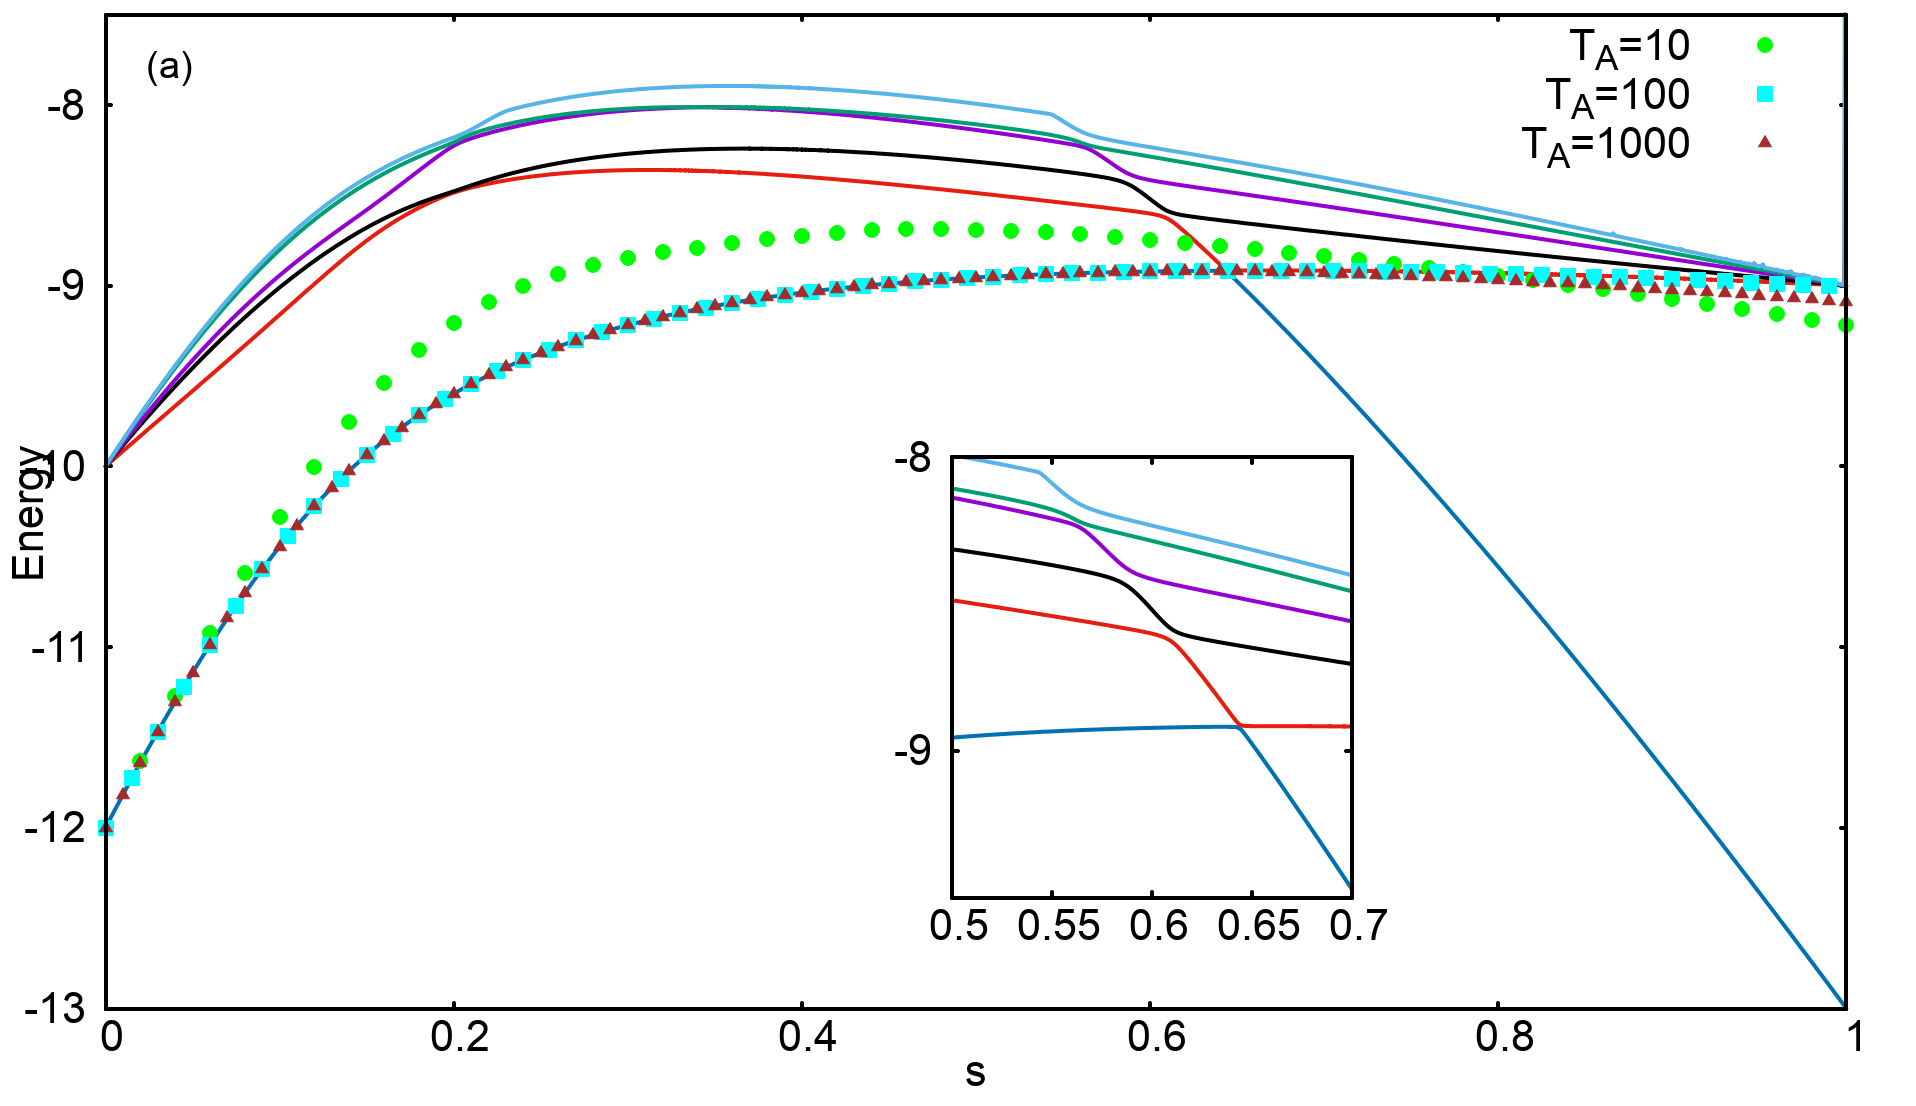
\includegraphics[scale=0.3]{950_s12_A_g0.png}
\caption{The energy spectrum for the second problem, with instantaneous energy values corresponding to three annealing times, with Anti-ferromagnetic trigger, and g=0.5. $\Delta_{min}$ was found to be 0.0130, while $p$=0.0022 for $T_A$=100. }
\label{fig:a4}
\end{figure}
\begin{figure}[H]
\centering 
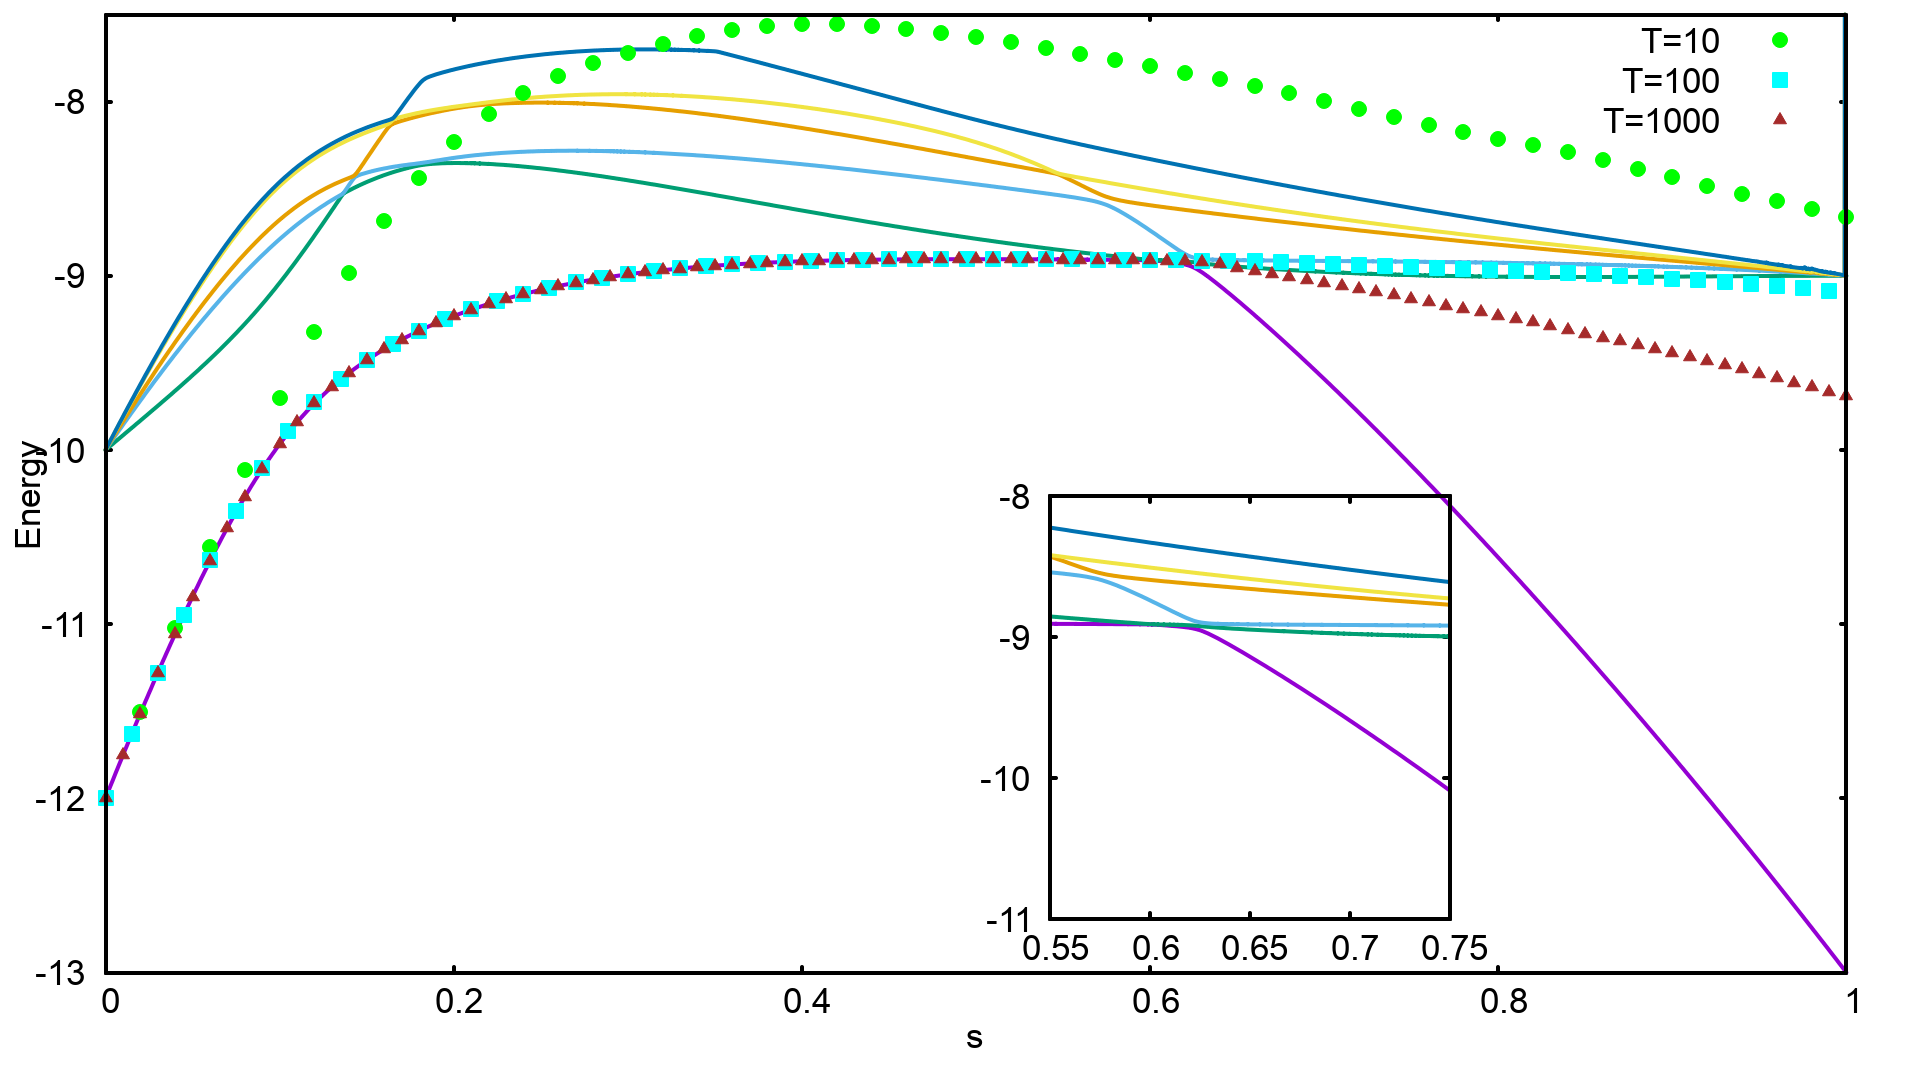
\includegraphics[scale=0.3]{950_s12_A_g1.png}
\caption{The energy spectrum for the second problem, with instantaneous energy values corresponding to three annealing times, with Anti-ferromagnetic trigger, and g=1. $\Delta_{min}$ was found to be 0.0019, while $p$=0.0239 for $T_A$=100. }
\label{fig:a5}
\end{figure}
\begin{figure}[H]
\centering 
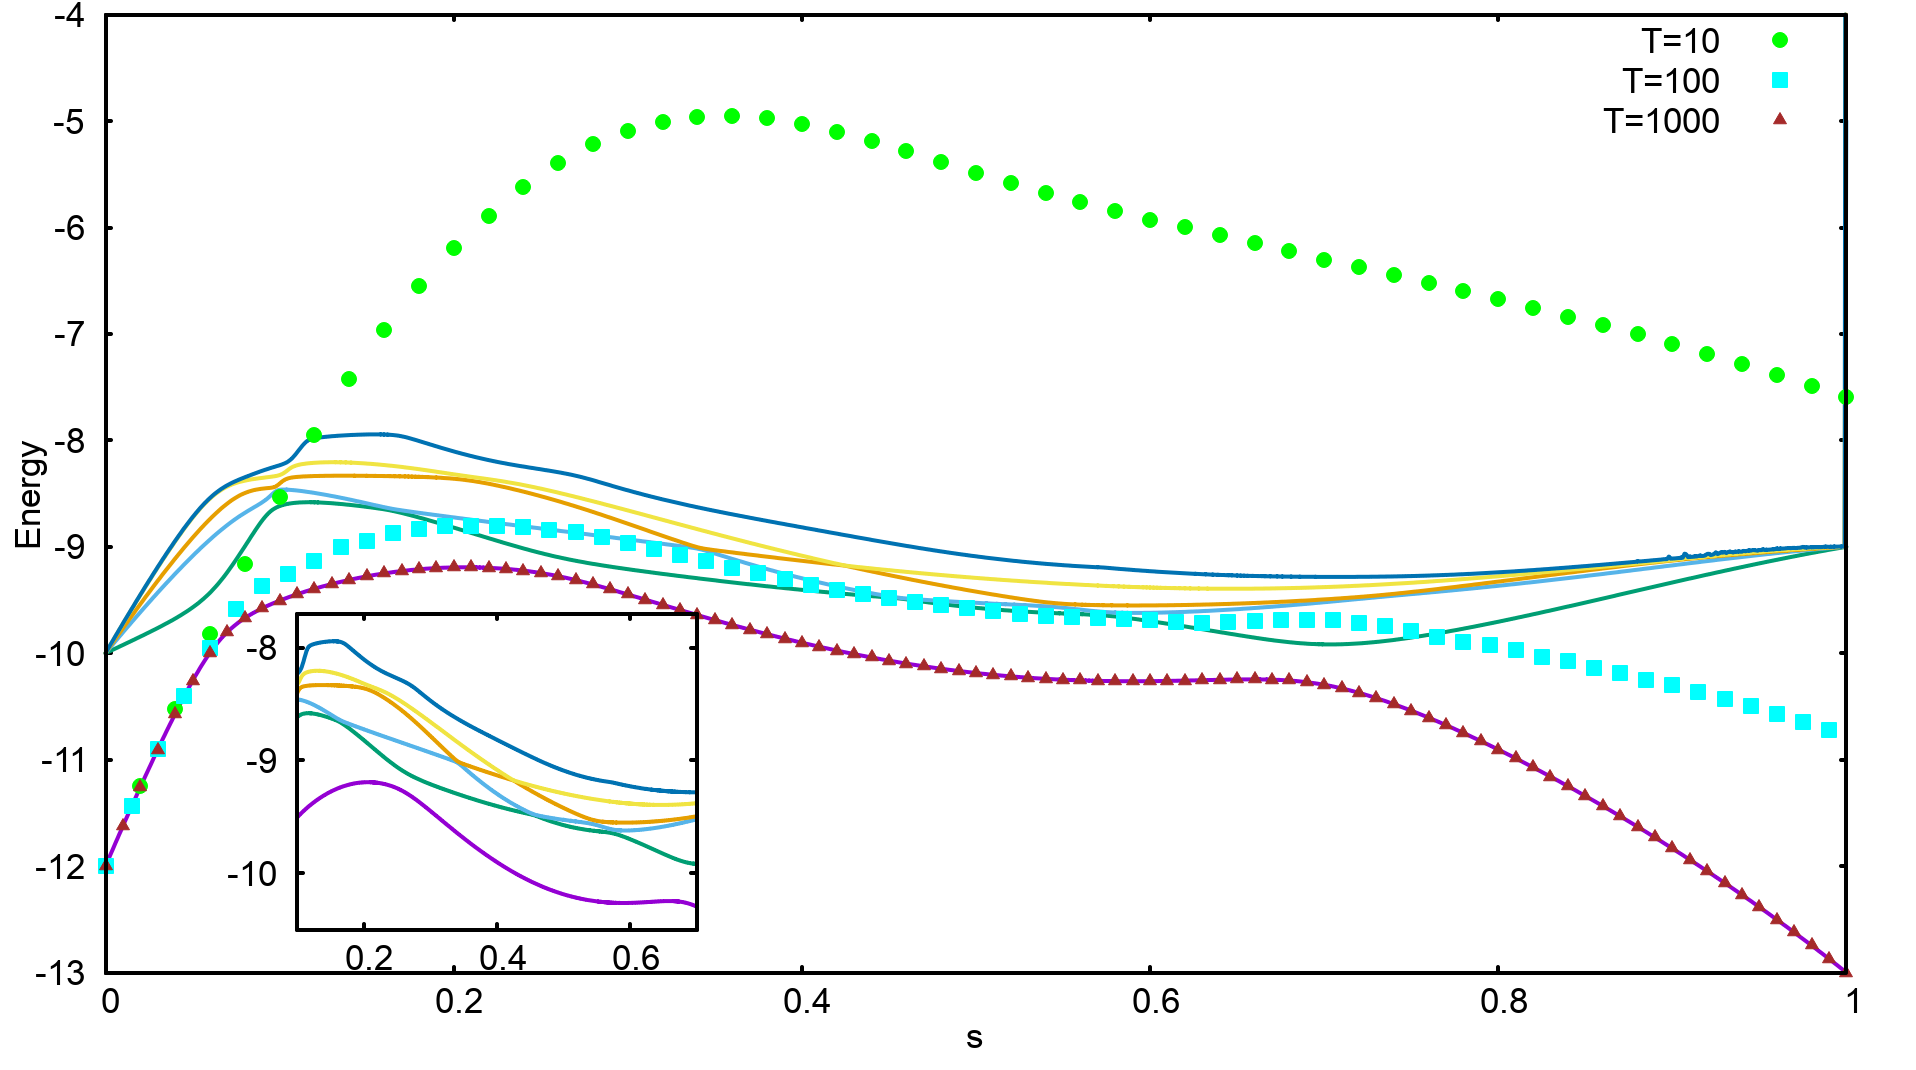
\includegraphics[scale=0.3]{950_s12_A_g2.png}
\caption{The energy spectrum for the second problem, with instantaneous energy values corresponding to three annealing times, with Anti-ferromagnetic trigger, and g=2. $\Delta_{min}$ was found to be 0.1784, while $p$=0.4468 for $T_A$=100. }
\label{fig:a6}
\end{figure}
For this case, table (\ref{tab:a2}) shows a comparison of the minimum energy gaps, and success probabilities (corresponding to different annealing times) between the original Hamiltonian and the Hamiltonian upon adding the anti-ferromagnetic trigger with different strengths. 

\begin{table}[H]
\centering
\renewcommand{\arraystretch}{1.5}
\begin{tabular}{|c|c|c|c|c|}
\hline 
CASE 2 & Original Hamiltonian & Trigger=A, g=0.5 & Trigger=A, g=1 & Trigger=A, g=2 \\ 
\hline 
$\Delta_{min}$ & 0.0312 & 0.0130 & 0.0019 & 0.1784 \\ 
\hline 
p($T_A$=10) & 2.343 $\times 10^{-4}$ & 0.0567 & 0.0017 & 0.0071\\ 
\hline 
p($T_A$=100) & 0.0146 & 0.0022 & 0.0239 & 0.4468 \\ 
\hline 
p($T_A$=1000) & 0.1362 & 0.0228 & 0.1729 & 0.9999 \\ 
\hline 
s value at $\Delta_{min}$ & 0.665 & 0.644 & 0.601 & 0.263 \\ 
\hline 
Number of anti-crossings & 1 & 1 & 2 & 3 \\
\hline
\end{tabular} 
\caption{A comparison of the minimum gaps and the success probabilities for the second chosen case, between the original Hamiltonian and and the Hamiltonian with anti-ferromagnetic trigger (A) of different strengths. The minimum gap becomes small for g=0.5, and even smaller for g=1, while it becomes even larger than the original minimum energy gap for g=2. The value of s corresponding to the position of the minimum gap becomes smaller with increasing strength of the trigger.}
\label{tab:a2}
\end{table}


The minimum energy gaps decrease with respect to the original energy gaps upon adding the trigger with strengths 0.5, and 1. However, the success probability at $T_A$=10 for anti-ferromagnetic trigger with g=0.5 and g=1 is larger compared to that of the original Hamiltonian, owing to different reasons.\\

Since upon adding the anti-ferromagnetic trigger with strength 0.5, the minimum energy gap becomes smaller, the annealing time of $T_A$=10 is so short that the state of the system transits to the first excited state even before the minimum gap anti-crossing. Upon approaching the minimum gap anti-crossing the system state shifts back to the ground state, increasing the success probability in this case (figure \ref{fig:a4}). However, for the original Hamiltonian the gap is large enough for an annealing time of 10 for the state to not shift to the first excited state before the minimum energy gap (figure \ref{fig:o3}). The state therefore stays close to the first excited state after crossing the anti-crossing.
Furthermore, for annealing times $T_A$=100 and $T_A$=1000, the system state transitions only at the minimum gap anti-crossing and closely follows the second and first excited states respectively. The overlap with the ground state decreases, and therefore the success probability for both these cases also reduces.\\

For the other case - with anti-ferromagnetic trigger with strength 1, the number of energy anti-crossings increases to 2. The first energy anti-crossing is small enough for just $T_A$=10 to shift the system state to the first excited state. Quickly after transitioning to the first excited state, the system state shifts to higher energy levels (figure \ref{fig:a5}). Since the state of the system is a superposition of all the energy eigenstates, the present state of system has small, yet finite overlap with the ground state. In the original Hamiltonian, however, the system state shifts to the first excited state at the only energy anti-crossing, and therefore the overlap with the ground state becomes negligible (figure \ref{fig:o3}).\\

By choosing the strength to be 2, the minimum energy gap of this problem becomes larger than the original minimum energy gap, while the number of anti-crossings between the ground and the first excited state increases to 3. The success probability in this case is always larger than the original success probability for all annealing times. For $T_A$=10, the state of the system shifts to the first excited state at first energy anti-crossing, and then quickly shifts to a superposition state with the higher energy states. This results in a larger overlap with the ground state compared to the case of the state closely following the first excited state after reaching the only energy anti-crossing in case of the original problem (\ref{fig:o3}).

For $T_A$=100, the state starts transitioning to the first excited state only as it approaches the second energy anti-crossing. The state does further shift to higher energy levels, but comes back to the first excited state before the third energy anti-crossing. After passing by the third anti-crossing some of the amplitude of the wave function shifts to the ground state again, and therefore the success becomes larger than the original problem. 


Finally, for $T_A$=1000, the annealing time and the minimum energy gap is large enough for the system to always stay close to the ground state, hence the larger success probability.\\

Lastly, figures (\ref{fig:a7}), (\ref{fig:a8}) and (\ref{fig:a9}) show the energy spectra and instantaneous energy values for the third problem, after adding the anti-ferromagnetic trigger with strengths 0.5, 1 and 2 respectively. 


\begin{figure}[H]
\centering 
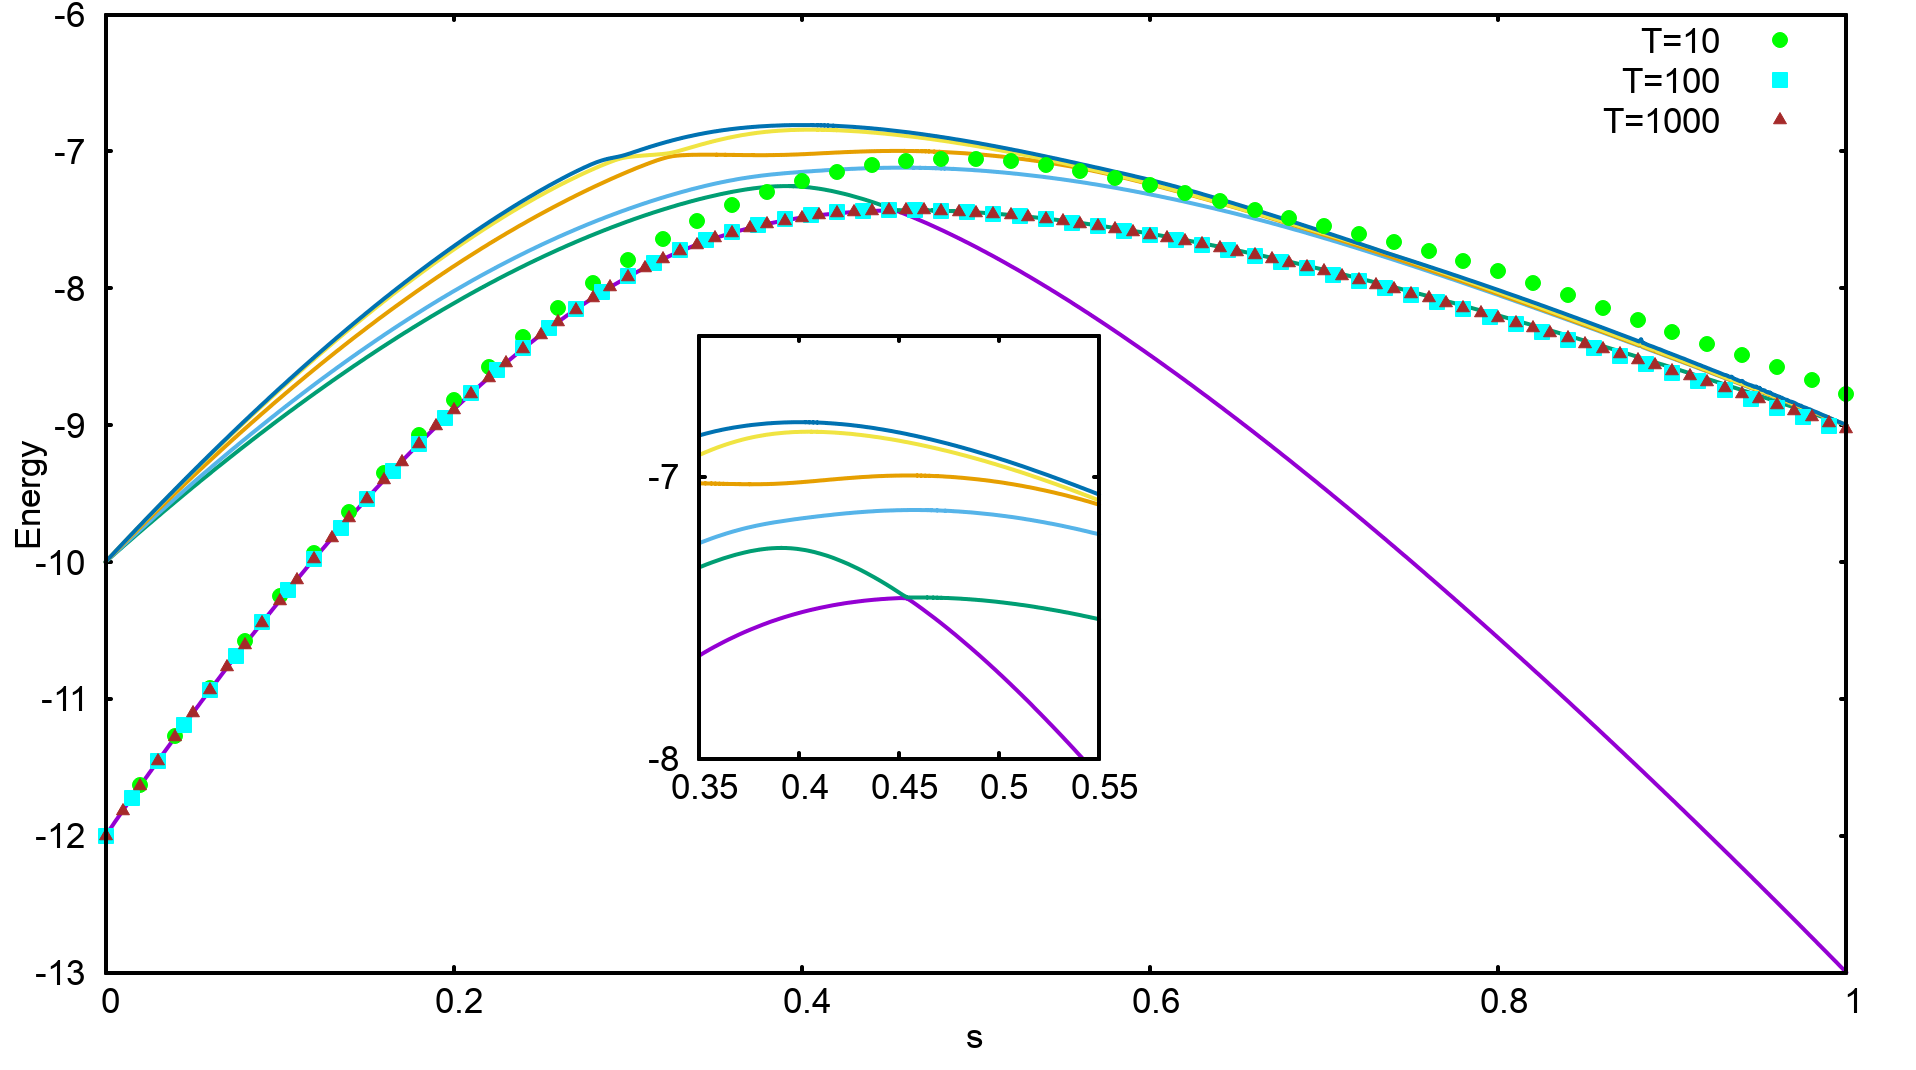
\includegraphics[scale=0.3]{528_s12_A_g0.png}
\caption{The energy spectrum for the third problem, with instantaneous energy values corresponding to three annealing times, with Anti-ferromagnetic trigger, and g=0.5. $\Delta_{min}$ was found to be 0.0049, while $p$=0.0120 for $T_A$=100. }
\label{fig:a7}
\end{figure}
\begin{figure}[H]
\centering 
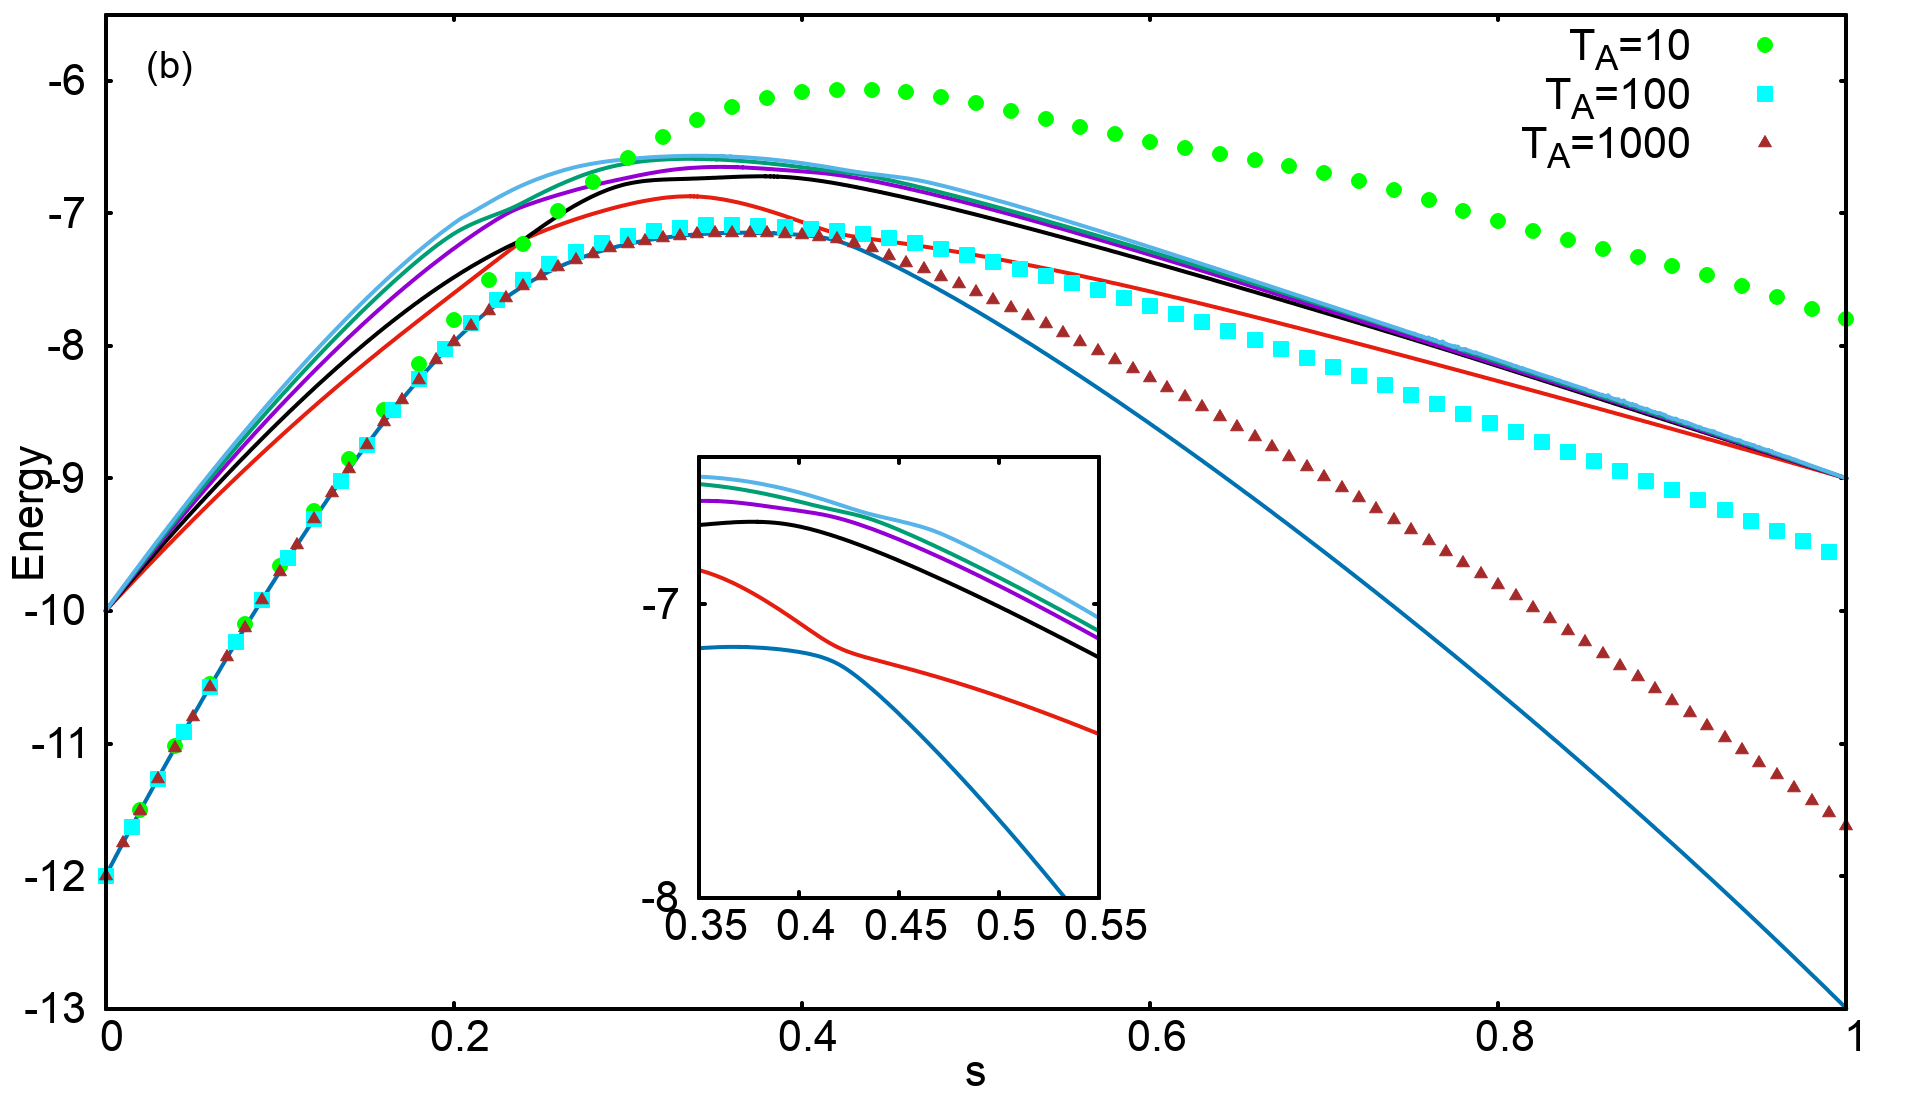
\includegraphics[scale=0.3]{528_s12_A_g1.png}
\caption{The energy spectrum for the third problem, with instantaneous energy values corresponding to three annealing times, with Anti-ferromagnetic trigger, and g=1. $\Delta_{min}$ was found to be 0.0562, while $p$=0.1517 for $T_A$=100. }
\label{fig:a8}
\end{figure}
\begin{figure}[H]
\centering 
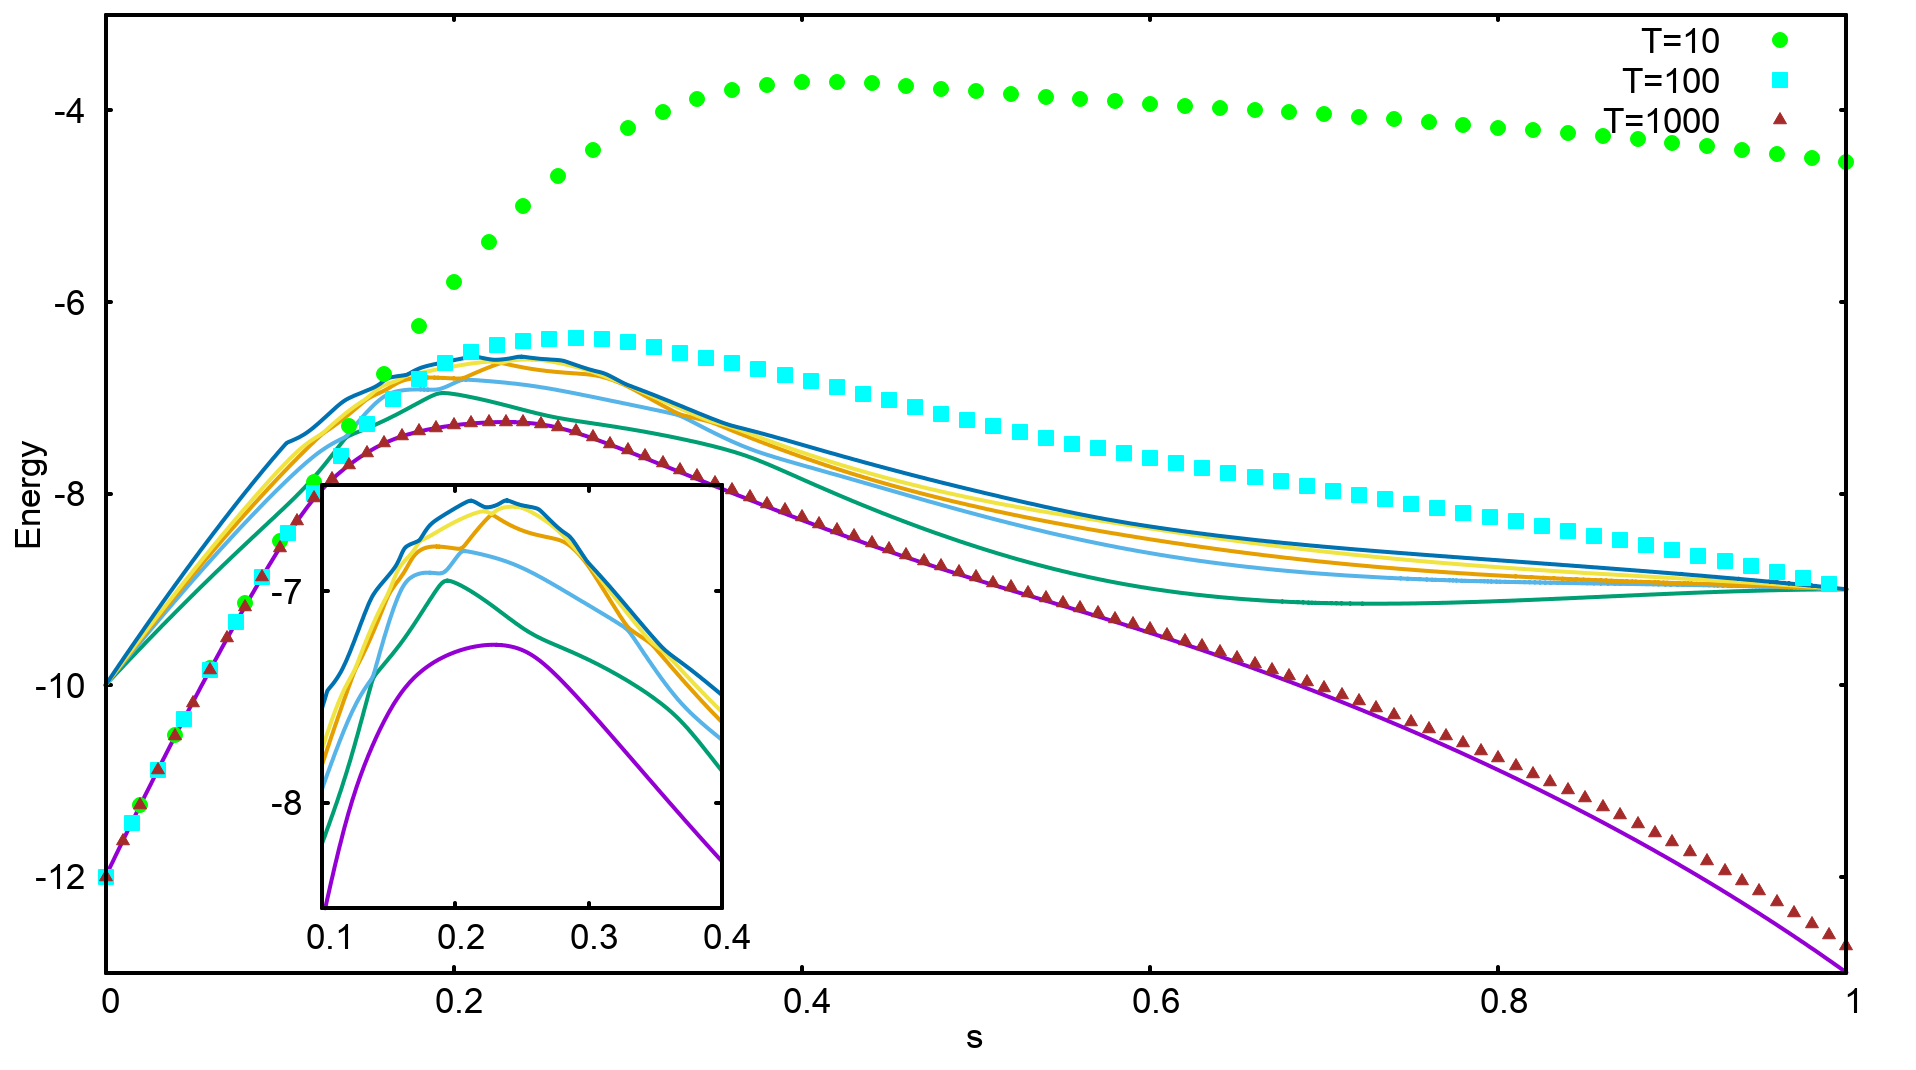
\includegraphics[scale=0.3]{528_s12_A_g2.png}
\caption{The energy spectrum for the third problem, with instantaneous energy values corresponding to three annealing times, with Anti-ferromagnetic trigger, and g=2. $\Delta_{min}$ was found to be 0.1008, while $p$=0.0480 for $T_A$=100. }
\label{fig:a9}
\end{figure}

Table (\ref{tab:a3}) shows a comparison of the minimum energy gaps, and success probabilities (corresponding to different annealing times) between the original Hamiltonian and the Hamiltonian upon adding the anti-ferromagnetic trigger with different strengths. 

\begin{table}[H]
\centering
\renewcommand{\arraystretch}{1.5}
\begin{tabular}{|c|c|c|c|c|}
\hline 
CASE 3 & Original Hamiltonian & Trigger=A, g=0.5 & Trigger=A, g=1 & Trigger=A, g=2 \\ 
\hline 
$\Delta_{min}$ & 0.1573 & 0.0049 & 0.0562 & 0.1008 \\ 
\hline 
p($T_A$=10) & 0.1577 & 0.0573 & 0.0368 & 4.21 $\times 10^{-5}$\\ 
\hline 
p($T_A$=100) & 0.5199 & 0.0120 & 0.1517 & 0.0480 \\ 
\hline 
p($T_A$=1000) & 0.9992 & 0.0071 & 0.6565 & 0.9313 \\ 
\hline 
s value at $\Delta_{min}$ & 0.514 & 0.454 & 0.418 & 0.256 \\ 
\hline 
Number of anti-crossings & 1 & 1 & 3 & 4 \\
\hline
\end{tabular} 
\caption{A comparison of the minimum gaps and the success probabilities for the third chosen case, between the original Hamiltonian and and the Hamiltonian with anti-ferromagnetic trigger (A) of different strengths. The minimum energy gaps after adding the trigger are smaller than the original minimum gap, for all the values of g. They however become large upon increasing the strength of the anti-ferromagnetic trigger. The value of s corresponding to the position of the minimum gap becomes smaller with increasing strength of the trigger.}
\label{tab:a3}
\end{table}

For this problem, it was observed that adding the anti-ferromagnetic trigger made the minimum energy gaps smaller than the original gap, for all the three values of the strength chosen. The gaps however increased with increasing the strength of the trigger. The original success probabilities, for all annealing times, are therefore larger than the resulting success probabilities upon adding the triggers with different g. Additionally, for all annealing times but $T_A$=10, the success probability become larger when the anti-ferromagnetic trigger is added with strength 1 compared to when added with strength 0.5, as the minimum energy gap for the former is larger. For $T_A$=10, and both g=0.5 and g=1 cases, the system state transitions to the first excited state prior to the first energy anti-crossing. This is followed by the state shifting to higher energy levels soon after. Since the energy spectrum becomes more complex (in terms of the number of anti-crossings between the higher energy states and the closeness of these states), as the strength of the trigger is increased, the state shifts farther away from the ground state as the strength of the trigger is increased. Consequently, the success probability decreases in the case with g=0.5.

 Although the gap becomes even larger for g=2, the success probability is smaller compared the case with g=1. This can be explained by observing that adding the anti-ferromagnetic trigger with g=2 changes the energy spectrum of the Hamiltonian even more drastically. Not only do the number of anti-crossings between the ground and the first excited state increase to 4, the higher lying energy levels also become more involved and have larger number of anti-crossings. Hence, as annealing times $T_A$=10 and $T_A$=100 are not large enough for the state to stay close to the ground state upon reaching the first energy anti-crossing, even farther away from the ground state as compared to the g=1 case. Hence, the success probability for $T_A$=10 and g=2 case is negligible. As the annealing time is increased further to $T_A$=1000, the minimum energy gap becomes large enough to keep the state of the system close to the ground state, and the success probability becomes comparable to the original success probability.
 
 
\section*{g=0.5}
This section will focus on the performance of the quantum annealing algorithm upon adding the anti-ferromagnetic trigger to each of the original Hamiltonian from 12-spin SAT problems, with strength 0.5. For each problem, annealing time was chosen to be 10, 100 and 1000. 

As a measure of quantifying the performance with respect to the original Hamiltonian, metrics Relative success probability was defined as the ratio of the success probability upon adding the anti-ferromagnetic trigger ($p^A$) to the original success probability ($p^O$). Figures (\ref{fig:a10}), (\ref{fig:a11}) and (\ref{fig:a12}) show the  distribution of the relative success probability for annealing times of 10, 100 and 1000 respectively. 

\begin{figure}[H]
\centering 
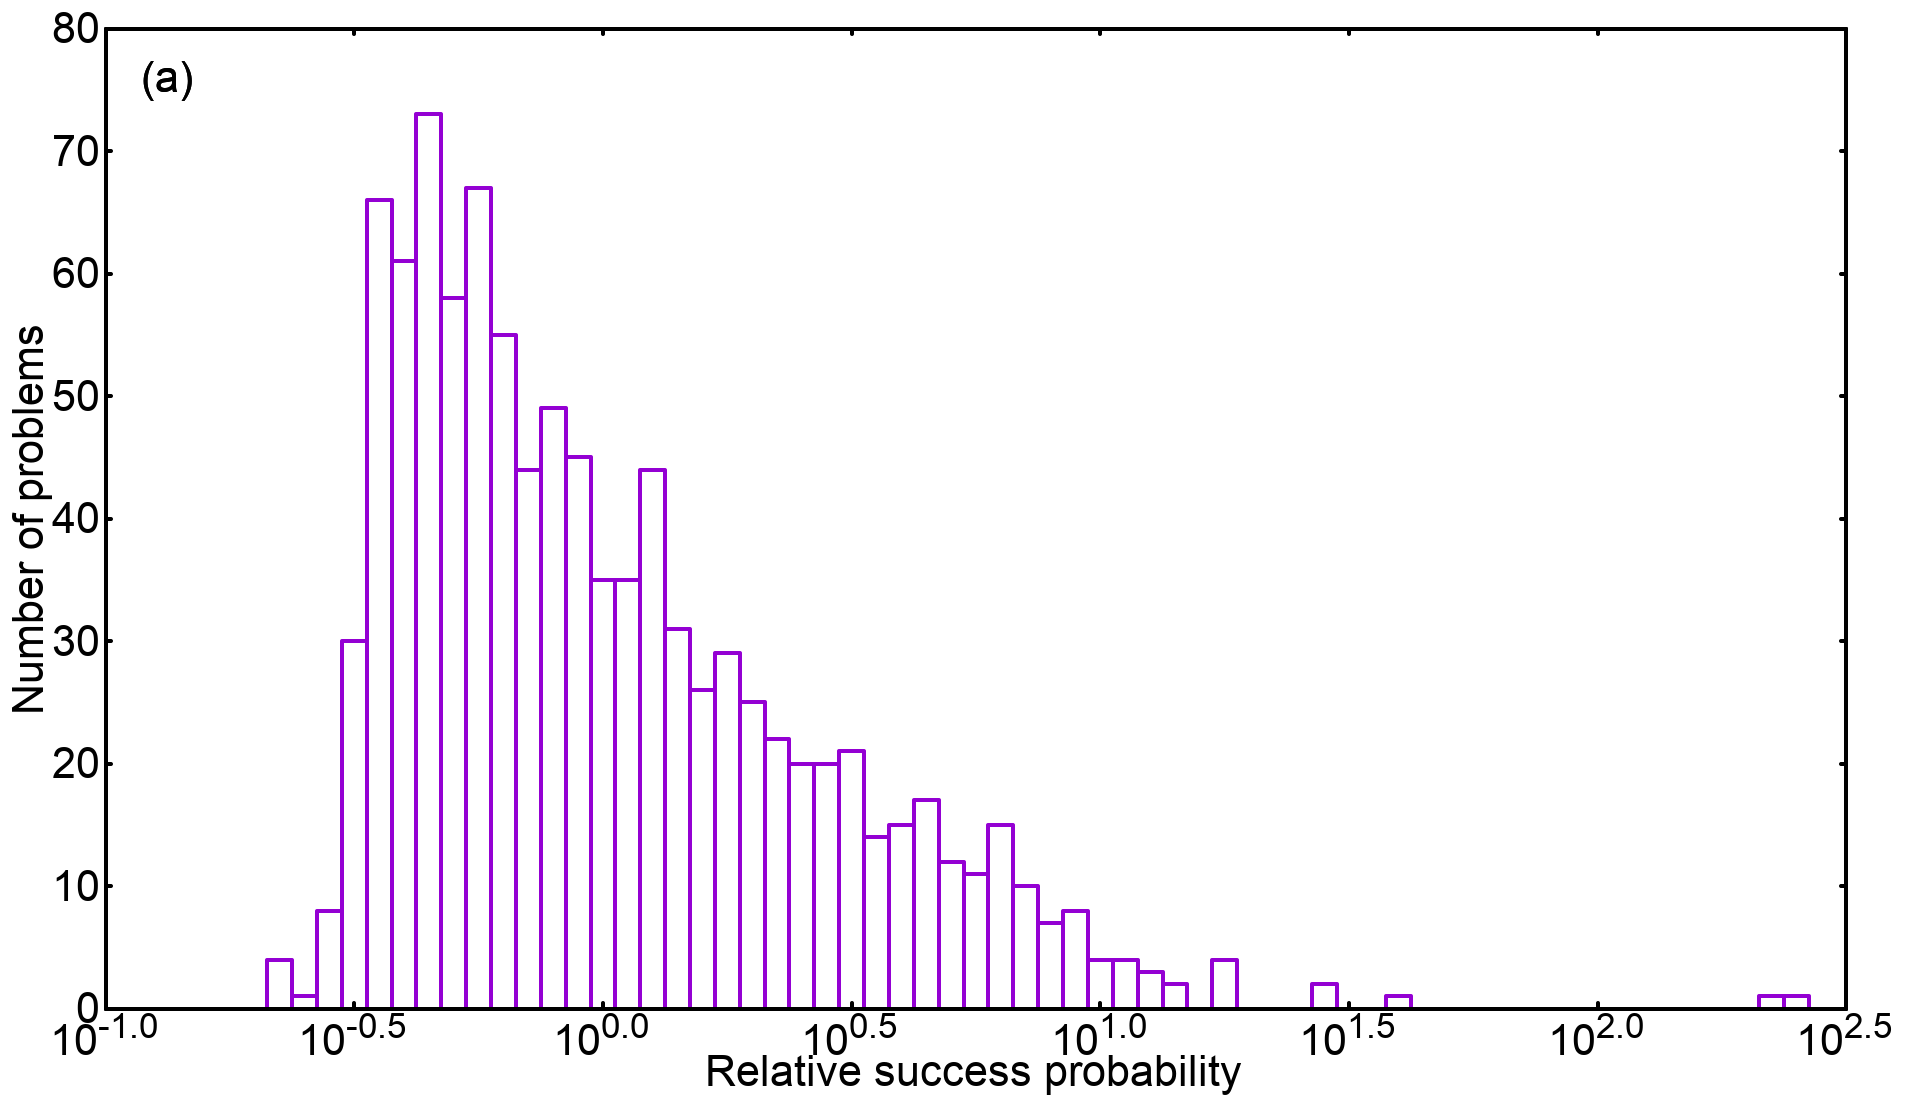
\includegraphics[scale=0.3]{A_T10_g0.png}
\caption{The distribution of relative success probability $\dfrac{p^A}{p^O}$for $T_A$=10. 43.9\% of the cases were found to have a higher success probability after adding the trigger.}
\label{fig:a10}
\end{figure}
\begin{figure}[H]
\centering 
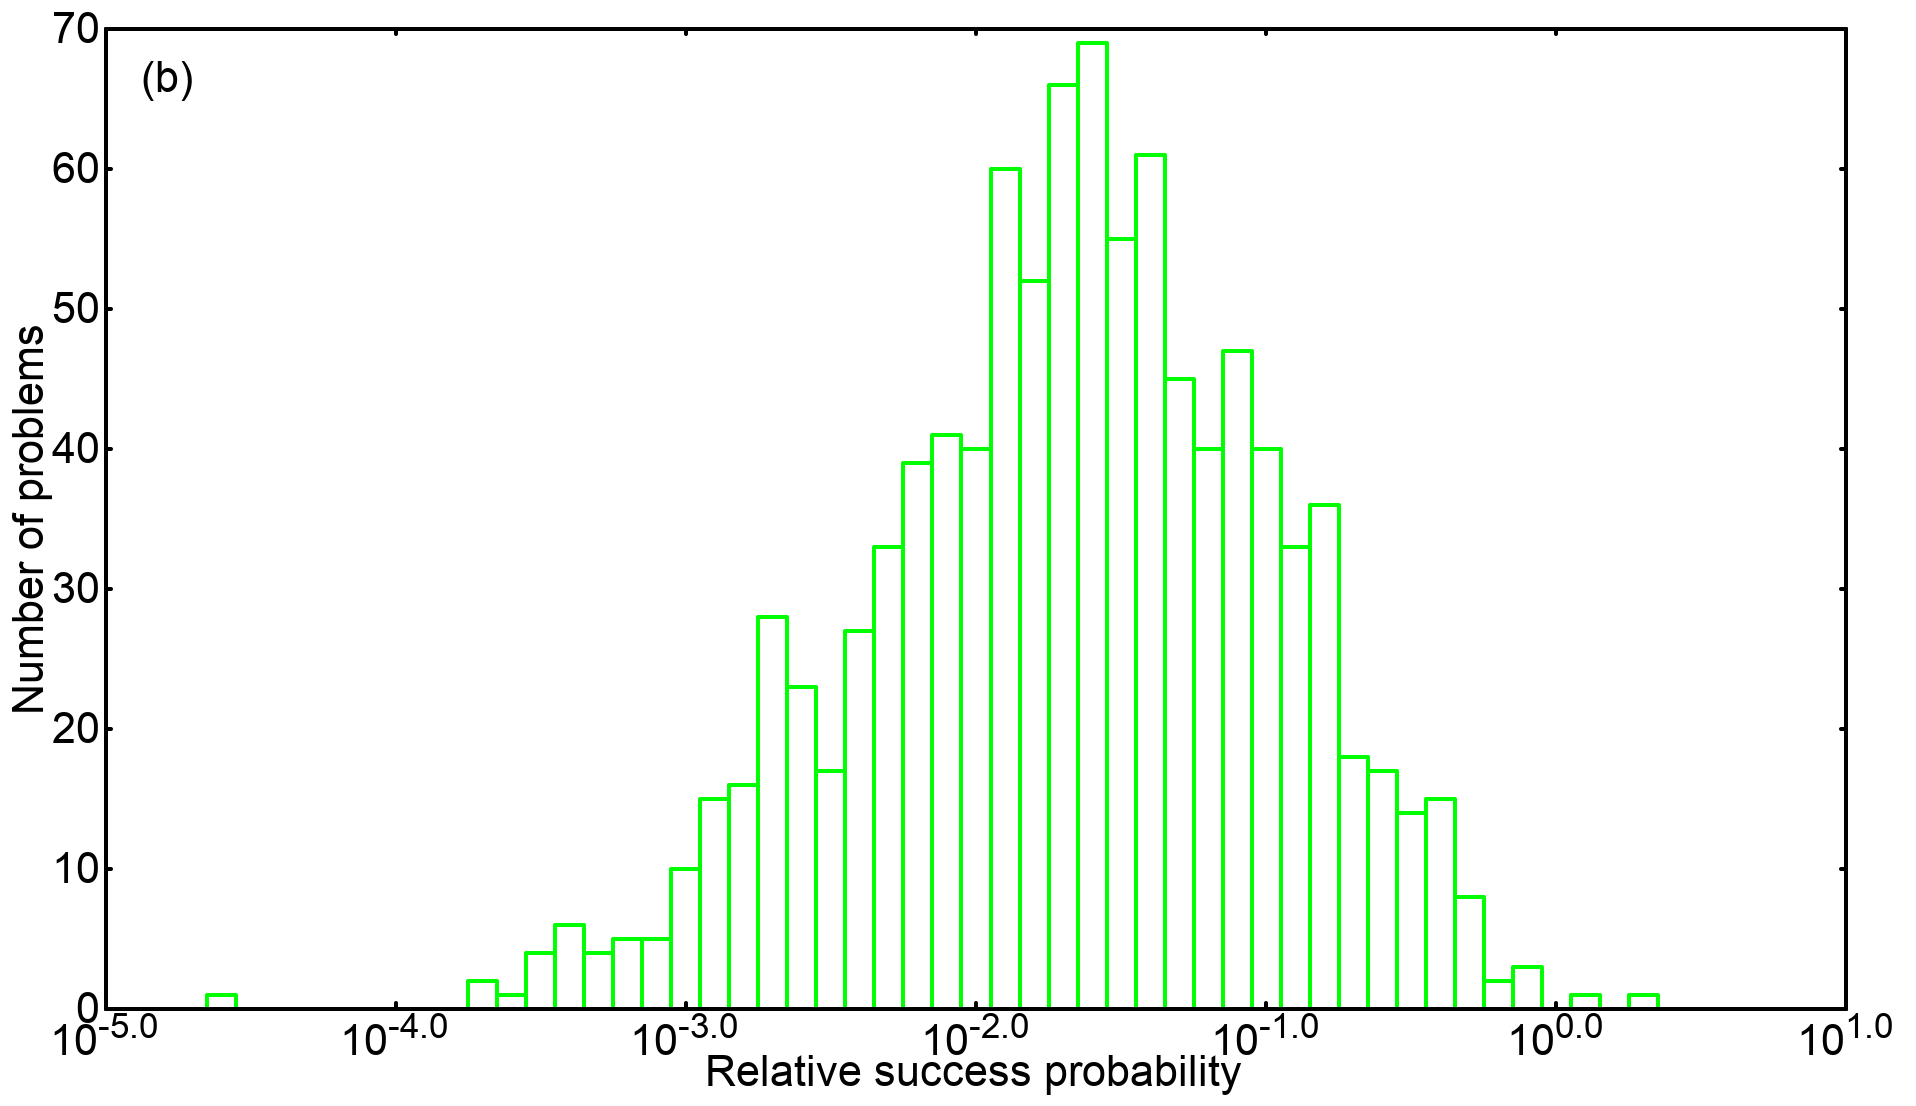
\includegraphics[scale=0.3]{A_T100_g0.png}
\caption{The distribution of relative success probability $\dfrac{p^A}{p^O}$for $T_A$=10. 0.2\% of the cases were found to have a higher success probability after adding the trigger. }
\label{fig:a11}
\end{figure}
\begin{figure}[H]
\centering 
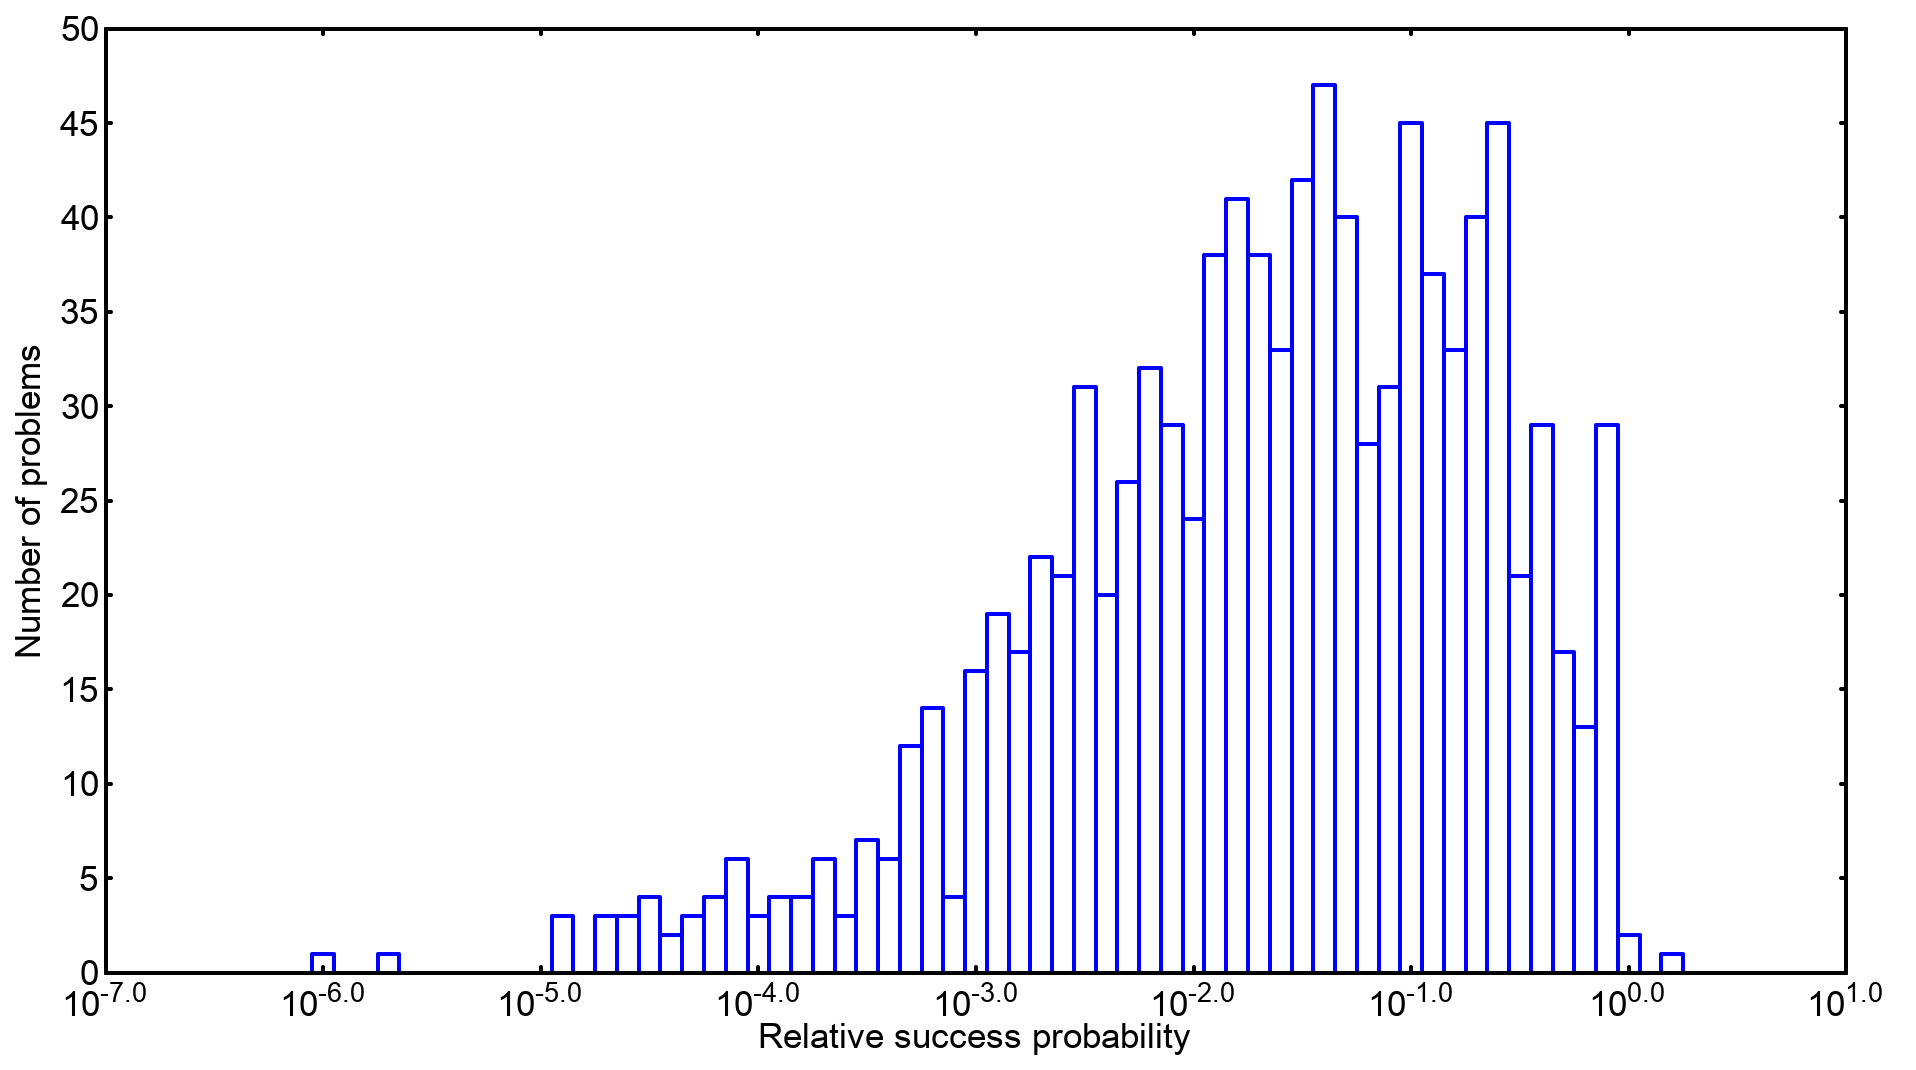
\includegraphics[scale=0.3]{A_T1000_g0.png}
\caption{The distribution of relative success probability $\dfrac{p^A}{p^O}$for $T_A$=10. 0.3\% of the cases were found to have a higher success probability after adding the trigger.}
\label{fig:a12}
\end{figure}

For an annealing time $T_A$=10, it was found that 43.9\% of the problems of the set were improved after the anti-ferromagnetic trigger with g=0.5. On increasing the annealing time to 100 and 1000, the percentage of cases with improved success probability dropped to 0.2\% and 0.3\% percent respectively. Furthermore, the largest value of the relative success ratio is a little more than 250 for $T_A$=10, while it reduces to 1.995 for $T_A$=100, and to 1.585 for $T_A$=1000. In order to understand the reasons for this decrease in the performance after adding the anti-ferromagnetic trigger, the minimum energy gaps of all the problems were calculated after adding the trigger. Figure (\ref{fig:a13}) shows a plot of the minimum energy gaps after adding the anti-ferromagnetic trigger ($\Delta_{min}^A$) with the original minimum energy gaps ($\Delta_{min}^O$).
\begin{figure}[H]
\centering 
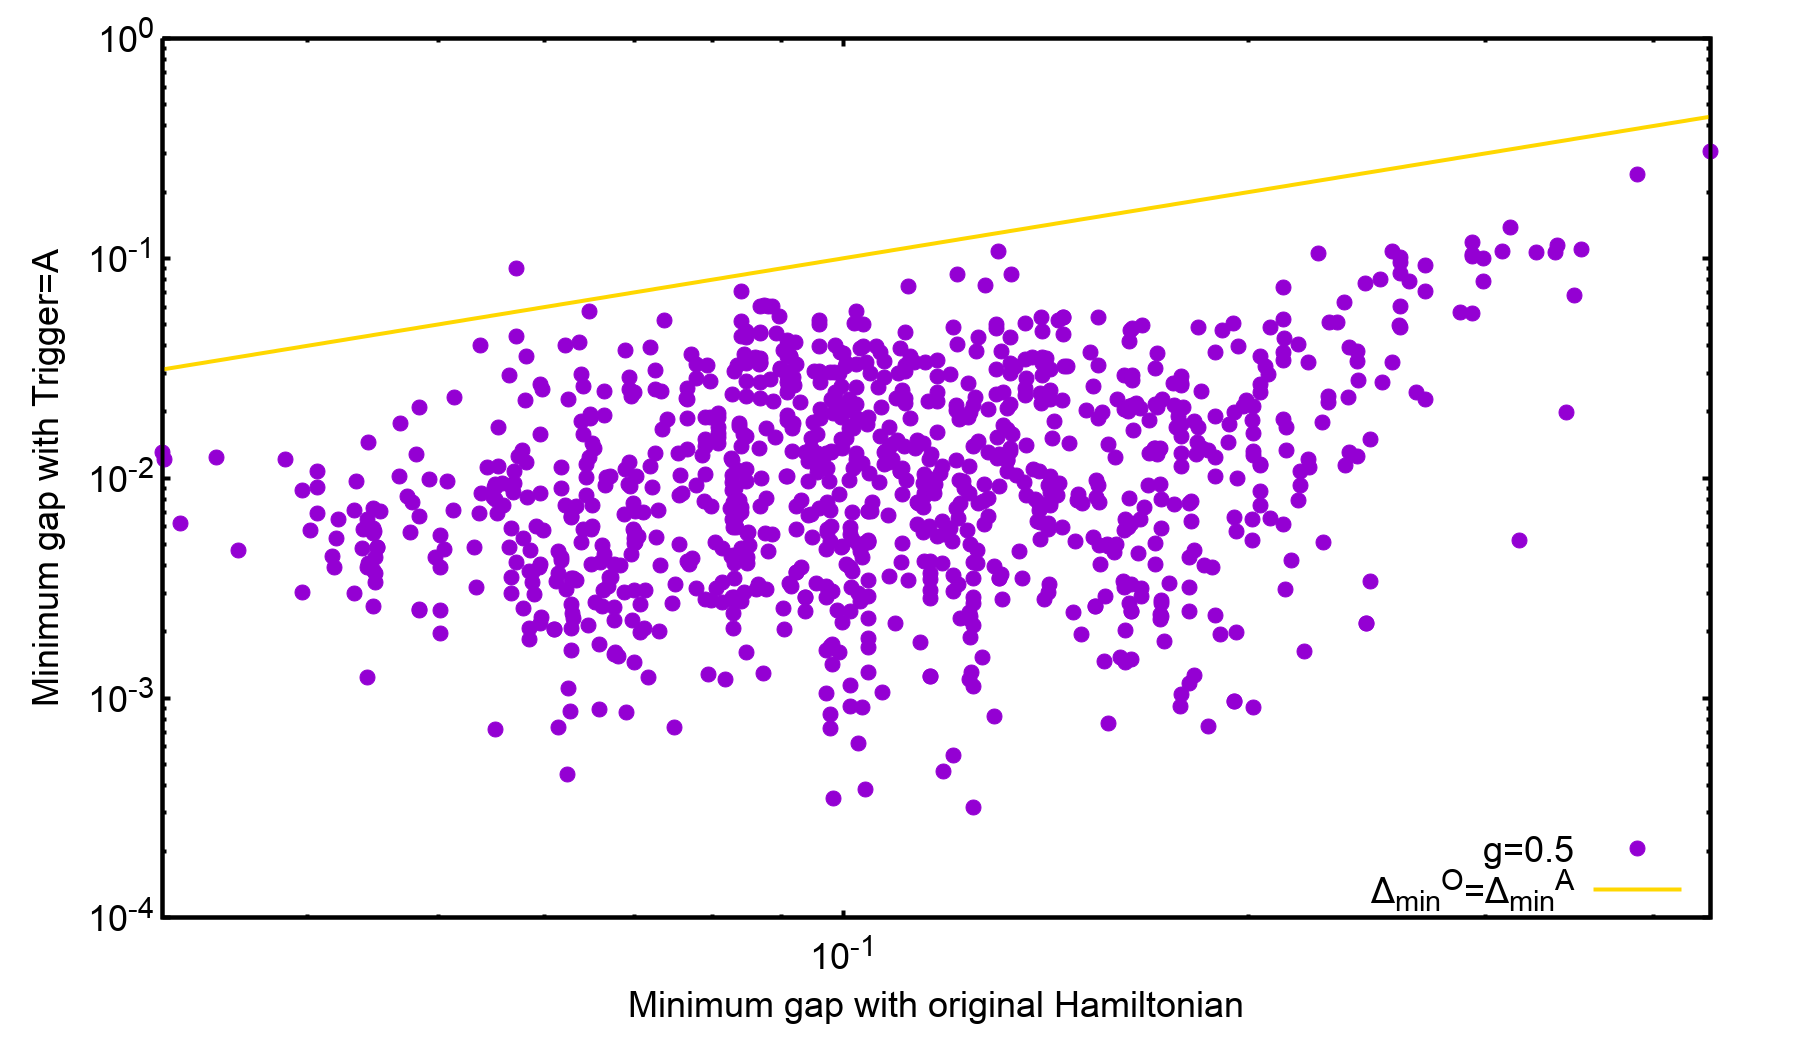
\includegraphics[scale=0.24]{MinGap_A_g0.png}
\caption{A plot of the minimum energy gaps after adding the anti-ferromagnetic trigger with g=0.5 ($\Delta_{min}^A$), with the original minimum energy gaps ($\Delta_{min}^O$). For 99.9\% of the minimum energy gap was found to have decreased after adding the trigger.}
\label{fig:a13}
\end{figure}
As is clear from figure (\ref{fig:a13}), for 99.9\% of the cases, the minimum energy gaps reduce after adding the anti-ferromagnetic trigger with strength 0.5. Additionally, 92.3\% of all the cases still had a single anti-crossing between the ground and the first excited state, while for the other 7.7\% of the cases, it increased to 2.

For shorter annealing times, like $T_A$=10, the success probability can benefit because of two reasons. As seen in the second chosen problem in the previous section, for small minimum energy gaps, and smaller annealing times, the state of the system can shift to the first excited state prior to the minimum gap anti-crossing. The overlap with the ground state can then increase because of the following reasons:
\begin{itemize}
\item If there no higher energy states close to the state of the system, the wave function of the state can transfer some amplitude back to the ground state.
\item If the higher energy states come close to the system state, before it approaches the energy anti-crossing, the system state can further transit to a superposition state of the higher energy levels. This might increase the overlap of the state with the ground state compared to the case where the state closely follows the first excited state after crossing the energy anti-crossing.
\end{itemize}

Thus, when the annealing time is increased to 100 or 1000, the state of the system stays close to the ground state till it reaches the energy anti-crossing, and transitions to the first excited state afterwards. This explains the drop in the percentage of improved cases upon increasing the annealing time and adding the anti-ferromagnetic trigger. \\

To get an estimate of the difficulty of the affected problems, figure (\ref{fig:a14} shows the scatter plots of the success probabilities after adding the trigger with the original success probabilities, for the three annealing times.

\begin{figure}[H]
\centering 
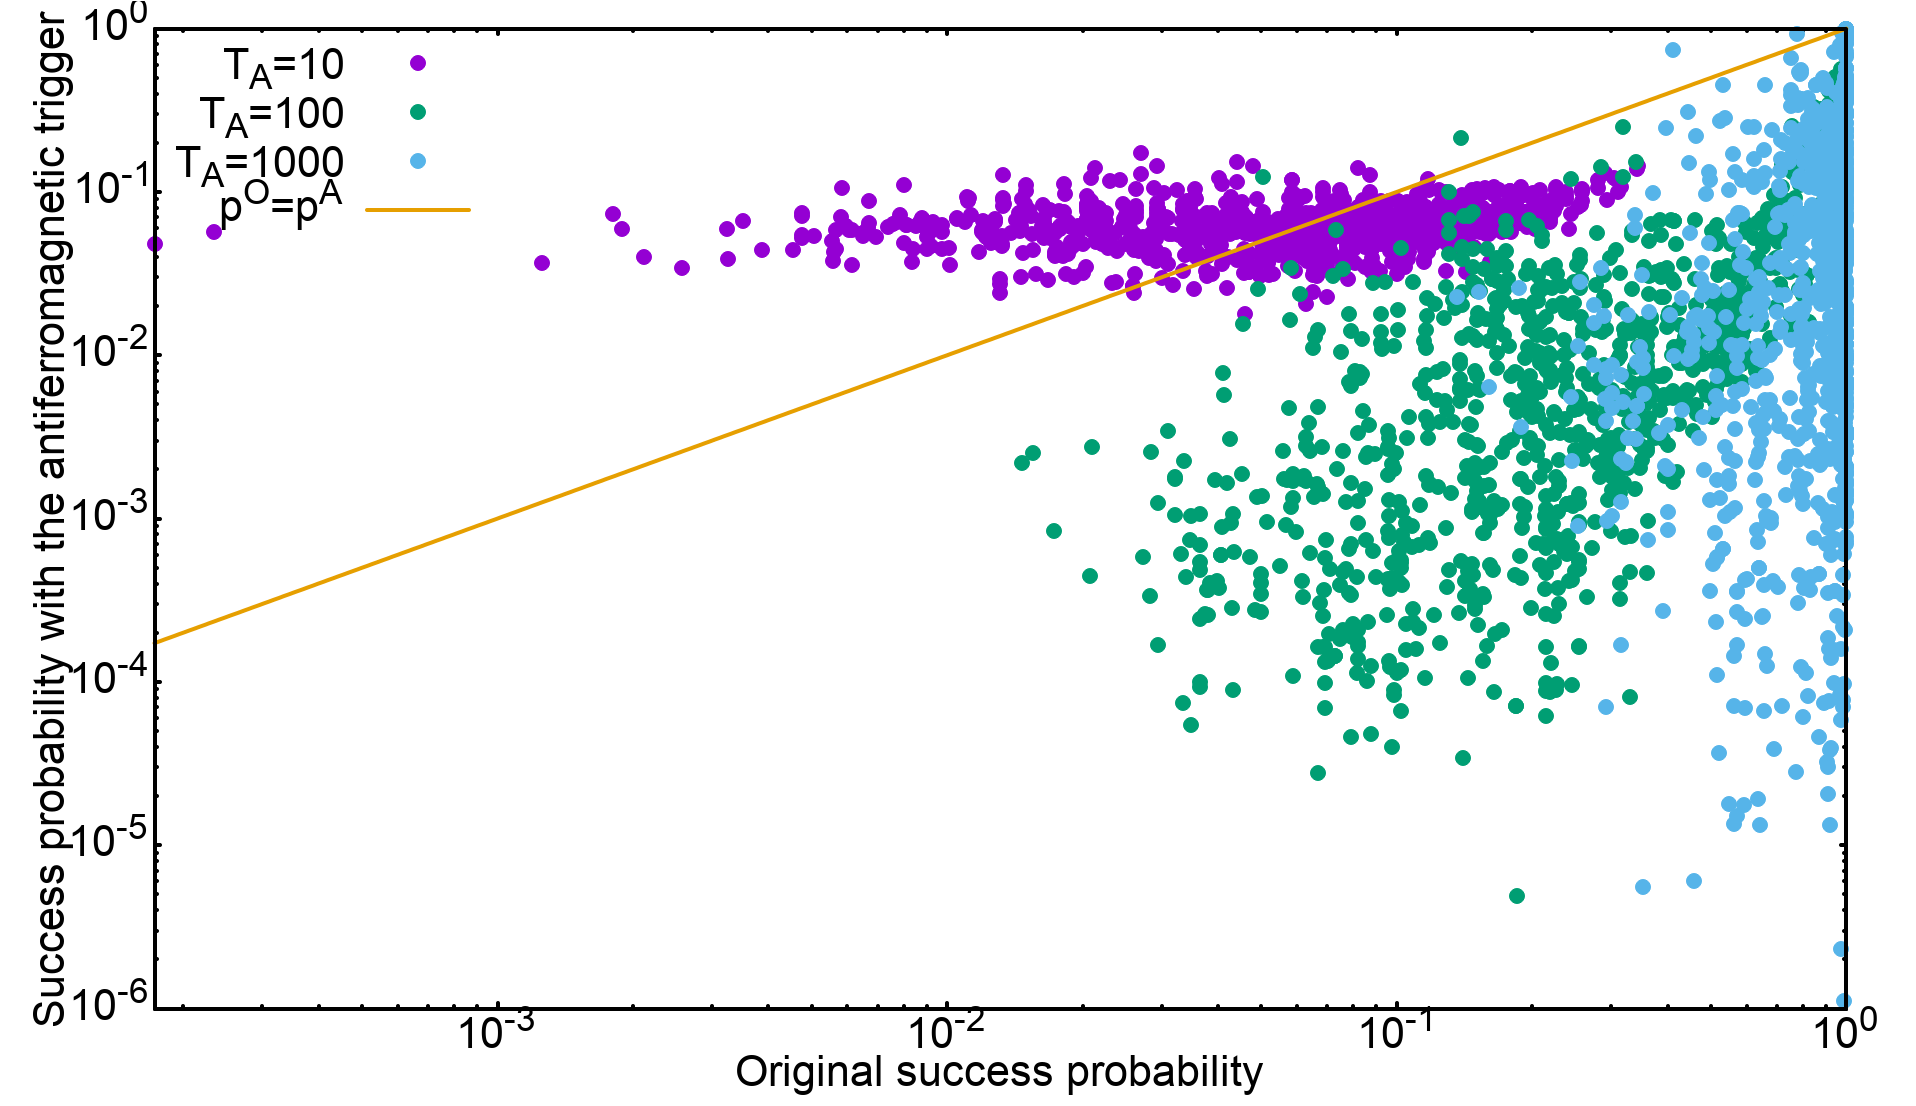
\includegraphics[scale=0.3]{ProbScat_g0.png}
\caption{A plot of the minimum energy gaps after adding the anti-ferromagnetic trigger with g=0.5 ($\Delta_{min}^A$), with the original minimum energy gaps ($\Delta_{min}^O$). For 99.9\% of the minimum energy gap was found to have decreased after adding the trigger.}
\label{fig:a13}
\end{figure}
\end{document}